\documentclass[twoside]{book}

% Packages required by doxygen
\usepackage{fixltx2e}
\usepackage{calc}
\usepackage{doxygen}
\usepackage[export]{adjustbox} % also loads graphicx
\usepackage{graphicx}
\usepackage[utf8]{inputenc}
\usepackage{makeidx}
\usepackage{multicol}
\usepackage{multirow}
\PassOptionsToPackage{warn}{textcomp}
\usepackage{textcomp}
\usepackage[nointegrals]{wasysym}
\usepackage[table]{xcolor}

% Font selection
\usepackage[T1]{fontenc}
\usepackage[scaled=.90]{helvet}
\usepackage{courier}
\usepackage{amssymb}
\usepackage{sectsty}
\renewcommand{\familydefault}{\sfdefault}
\allsectionsfont{%
  \fontseries{bc}\selectfont%
  \color{darkgray}%
}
\renewcommand{\DoxyLabelFont}{%
  \fontseries{bc}\selectfont%
  \color{darkgray}%
}
\newcommand{\+}{\discretionary{\mbox{\scriptsize$\hookleftarrow$}}{}{}}

% Page & text layout
\usepackage{geometry}
\geometry{%
  a4paper,%
  top=2.5cm,%
  bottom=2.5cm,%
  left=2.5cm,%
  right=2.5cm%
}
\tolerance=750
\hfuzz=15pt
\hbadness=750
\setlength{\emergencystretch}{15pt}
\setlength{\parindent}{0cm}
\setlength{\parskip}{3ex plus 2ex minus 2ex}
\makeatletter
\renewcommand{\paragraph}{%
  \@startsection{paragraph}{4}{0ex}{-1.0ex}{1.0ex}{%
    \normalfont\normalsize\bfseries\SS@parafont%
  }%
}
\renewcommand{\subparagraph}{%
  \@startsection{subparagraph}{5}{0ex}{-1.0ex}{1.0ex}{%
    \normalfont\normalsize\bfseries\SS@subparafont%
  }%
}
\makeatother

% Headers & footers
\usepackage{fancyhdr}
\pagestyle{fancyplain}
\fancyhead[LE]{\fancyplain{}{\bfseries\thepage}}
\fancyhead[CE]{\fancyplain{}{}}
\fancyhead[RE]{\fancyplain{}{\bfseries\leftmark}}
\fancyhead[LO]{\fancyplain{}{\bfseries\rightmark}}
\fancyhead[CO]{\fancyplain{}{}}
\fancyhead[RO]{\fancyplain{}{\bfseries\thepage}}
\fancyfoot[LE]{\fancyplain{}{}}
\fancyfoot[CE]{\fancyplain{}{}}
\fancyfoot[RE]{\fancyplain{}{\bfseries\scriptsize Generated by Doxygen }}
\fancyfoot[LO]{\fancyplain{}{\bfseries\scriptsize Generated by Doxygen }}
\fancyfoot[CO]{\fancyplain{}{}}
\fancyfoot[RO]{\fancyplain{}{}}
\renewcommand{\footrulewidth}{0.4pt}
\renewcommand{\chaptermark}[1]{%
  \markboth{#1}{}%
}
\renewcommand{\sectionmark}[1]{%
  \markright{\thesection\ #1}%
}

% Indices & bibliography
\usepackage{natbib}
\usepackage[titles]{tocloft}
\setcounter{tocdepth}{3}
\setcounter{secnumdepth}{5}
\makeindex

% Hyperlinks (required, but should be loaded last)
\usepackage{ifpdf}
\ifpdf
  \usepackage[pdftex,pagebackref=true]{hyperref}
\else
  \usepackage[ps2pdf,pagebackref=true]{hyperref}
\fi
\hypersetup{%
  colorlinks=true,%
  linkcolor=blue,%
  citecolor=blue,%
  unicode%
}

% Custom commands
\newcommand{\clearemptydoublepage}{%
  \newpage{\pagestyle{empty}\cleardoublepage}%
}

\usepackage{caption}
\captionsetup{labelsep=space,justification=centering,font={bf},singlelinecheck=off,skip=4pt,position=top}

%===== C O N T E N T S =====

\begin{document}

% Titlepage & ToC
\hypersetup{pageanchor=false,
             bookmarksnumbered=true,
             pdfencoding=unicode
            }
\pagenumbering{roman}
\begin{titlepage}
\vspace*{7cm}
\begin{center}%
{\Large Beroepsproduct World Robot Interface \\[1ex]\large 0.\+1 }\\
\vspace*{1cm}
{\large Generated by Doxygen 1.8.11}\\
\end{center}
\end{titlepage}
\clearemptydoublepage
\tableofcontents
\clearemptydoublepage
\pagenumbering{arabic}
\hypersetup{pageanchor=true}

%--- Begin generated contents ---
\chapter{Class Index}
\section{Class List}
Here are the classes, structs, unions and interfaces with brief descriptions\+:\begin{DoxyCompactList}
\item\contentsline{section}{\hyperlink{class_motion_control}{Motion\+Control} }{\pageref{class_motion_control}}{}
\item\contentsline{section}{\hyperlink{class_movement_command}{Movement\+Command} }{\pageref{class_movement_command}}{}
\item\contentsline{section}{\hyperlink{class_ros_communication}{Ros\+Communication} }{\pageref{class_ros_communication}}{}
\item\contentsline{section}{\hyperlink{class_serial_control}{Serial\+Control} }{\pageref{class_serial_control}}{}
\item\contentsline{section}{\hyperlink{class_servo}{Servo} }{\pageref{class_servo}}{}
\item\contentsline{section}{\hyperlink{class_smart_queue}{Smart\+Queue$<$ T $>$} }{\pageref{class_smart_queue}}{}
\end{DoxyCompactList}

\chapter{File Index}
\section{File List}
Here is a list of all files with brief descriptions\+:\begin{DoxyCompactList}
\item\contentsline{section}{\hyperlink{main_8cpp}{main.\+cpp} }{\pageref{main_8cpp}}{}
\item\contentsline{section}{\hyperlink{_motion_control_8cpp}{Motion\+Control.\+cpp} }{\pageref{_motion_control_8cpp}}{}
\item\contentsline{section}{\hyperlink{_motion_control_8hpp}{Motion\+Control.\+hpp} }{\pageref{_motion_control_8hpp}}{}
\item\contentsline{section}{\hyperlink{_movement_command_8hpp}{Movement\+Command.\+hpp} }{\pageref{_movement_command_8hpp}}{}
\item\contentsline{section}{\hyperlink{_ros_communication_8cpp}{Ros\+Communication.\+cpp} }{\pageref{_ros_communication_8cpp}}{}
\item\contentsline{section}{\hyperlink{_ros_communication_8hpp}{Ros\+Communication.\+hpp} }{\pageref{_ros_communication_8hpp}}{}
\item\contentsline{section}{\hyperlink{_serial_control_8cpp}{Serial\+Control.\+cpp} }{\pageref{_serial_control_8cpp}}{}
\item\contentsline{section}{\hyperlink{_serial_control_8hpp}{Serial\+Control.\+hpp} }{\pageref{_serial_control_8hpp}}{}
\item\contentsline{section}{\hyperlink{_servo_8hpp}{Servo.\+hpp} }{\pageref{_servo_8hpp}}{}
\item\contentsline{section}{\hyperlink{_smart_queue_8hpp}{Smart\+Queue.\+hpp} }{\pageref{_smart_queue_8hpp}}{}
\end{DoxyCompactList}

\chapter{Class Documentation}
\hypertarget{class_motion_control}{}\section{Motion\+Control Class Reference}
\label{class_motion_control}\index{Motion\+Control@{Motion\+Control}}


{\ttfamily \#include $<$Motion\+Control.\+hpp$>$}



Collaboration diagram for Motion\+Control\+:
\nopagebreak
\begin{figure}[H]
\begin{center}
\leavevmode
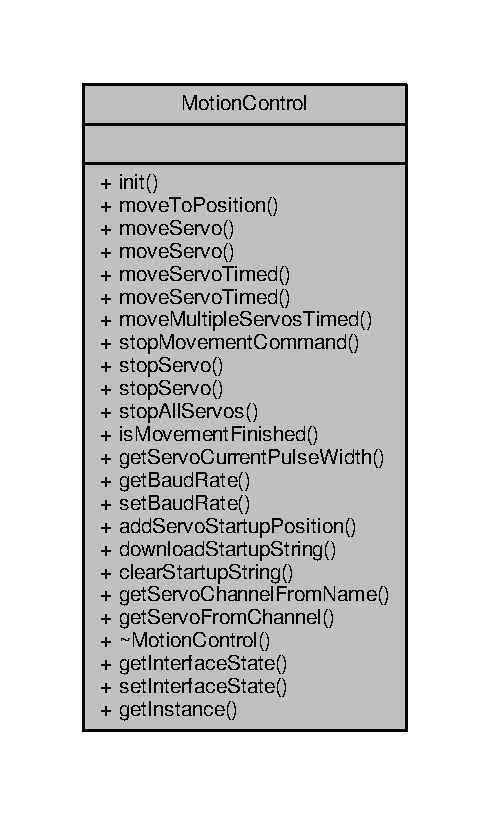
\includegraphics[width=235pt]{class_motion_control__coll__graph}
\end{center}
\end{figure}
\subsection*{Public Member Functions}
\begin{DoxyCompactItemize}
\item 
bool \hyperlink{class_motion_control_af101a2f120d4e5a08c540d83ef078768}{init} ()
\begin{DoxyCompactList}\small\item\em Starts the initialization of the motion controller. \end{DoxyCompactList}\item 
void \hyperlink{class_motion_control_ae348a531c3fe5a5d8d729e1dd2387f7f}{move\+To\+Position} (\hyperlink{_motion_control_8hpp_ac70e3c2821eb6a3860441f2c682f0aa4}{default\+Positions} position)
\begin{DoxyCompactList}\small\item\em Moves robot to a predefined position. \end{DoxyCompactList}\item 
void \hyperlink{class_motion_control_a69e807208c6fffd7c4b7c7159792c3e9}{move\+Servo} (const uint8\+\_\+t channel, const uint16\+\_\+t rotation, const uint16\+\_\+t speed)
\begin{DoxyCompactList}\small\item\em Moves a single servo with a specific speed. \end{DoxyCompactList}\item 
void \hyperlink{class_motion_control_a0acba77f349d42609ed2c0e520b8cf08}{move\+Servo} (const std\+::string name, const uint16\+\_\+t rotation, const uint16\+\_\+t speed)
\begin{DoxyCompactList}\small\item\em Moves a single servo with a specific speed. \end{DoxyCompactList}\item 
void \hyperlink{class_motion_control_a13582b1d506a7e85b23efaa9750ba0c8}{move\+Servo\+Timed} (const uint8\+\_\+t channel, const uint16\+\_\+t rotation, const uint16\+\_\+t time)
\begin{DoxyCompactList}\small\item\em Moves a single servo in a spcified time. \end{DoxyCompactList}\item 
void \hyperlink{class_motion_control_af2e8c8ede76ded5423deeddffa20ea52}{move\+Servo\+Timed} (const std\+::string name, const uint16\+\_\+t rotation, const uint16\+\_\+t time)
\begin{DoxyCompactList}\small\item\em Moves a single servo in a spcified time. \end{DoxyCompactList}\item 
void \hyperlink{class_motion_control_ab0693a90571a5e641cb7a7f8d43cee7a}{move\+Multiple\+Servos\+Timed} (const std\+::vector$<$ std\+::pair$<$ uint8\+\_\+t, uint16\+\_\+t $>$$>$ servo\+Positions, const uint16\+\_\+t time)
\begin{DoxyCompactList}\small\item\em Sends a movement command that moves multiple servo\textquotesingle{}s at once to a location. \end{DoxyCompactList}\item 
void \hyperlink{class_motion_control_aef8ec3f50c56b8981114c742486adae9}{stop\+Movement\+Command} (const uint8\+\_\+t channel)
\begin{DoxyCompactList}\small\item\em Stops all the movement that is currently going on. \end{DoxyCompactList}\item 
void \hyperlink{class_motion_control_a620288ede2a839574451dcfa5ff9c923}{stop\+Servo} (const uint8\+\_\+t channel)
\begin{DoxyCompactList}\small\item\em Immidetly stops servo. \end{DoxyCompactList}\item 
void \hyperlink{class_motion_control_af8136756f3c37e8d7850b3f320661e34}{stop\+Servo} (const std\+::string name)
\begin{DoxyCompactList}\small\item\em Immidetly stops servo. \end{DoxyCompactList}\item 
void \hyperlink{class_motion_control_ac45a88fcd3c1f1b238260ae8d1cb020f}{stop\+All\+Servos} ()
\begin{DoxyCompactList}\small\item\em Stops all connected servo\textquotesingle{}s immidietly. \end{DoxyCompactList}\item 
bool \hyperlink{class_motion_control_aee4432cb6495fb8c4ca87aede785a279}{is\+Movement\+Finished} ()
\begin{DoxyCompactList}\small\item\em Checks if the last movement command has been finished. \end{DoxyCompactList}\item 
uint16\+\_\+t \hyperlink{class_motion_control_ace0441eb6ebd0746a7cd725888eda95f}{get\+Servo\+Current\+Pulse\+Width} (const uint8\+\_\+t channel)
\begin{DoxyCompactList}\small\item\em Gets the servo current pulse width. \end{DoxyCompactList}\item 
uint32\+\_\+t \hyperlink{class_motion_control_a8285160feb7216da095011467e89296a}{get\+Baud\+Rate} ()
\begin{DoxyCompactList}\small\item\em Gets baudrate from C\+S\+S-\/32U. \end{DoxyCompactList}\item 
void \hyperlink{class_motion_control_a1fff14f3ca9bb02e88c1732d99ed85da}{set\+Baud\+Rate} (uint32\+\_\+t baud\+Rate)
\begin{DoxyCompactList}\small\item\em Sets the bautrate of the C\+S\+S-\/32U. \end{DoxyCompactList}\item 
void \hyperlink{class_motion_control_a4f4f1db6889e853aa8f65d9798ed82f9}{add\+Servo\+Startup\+Position} (const uint8\+\_\+t channel, const uint16\+\_\+t degrees, const uint16\+\_\+t speed)
\begin{DoxyCompactList}\small\item\em Adds a servo movement command to the end of the startup string. \end{DoxyCompactList}\item 
void \hyperlink{class_motion_control_a75a6ade7872ae6dca9a9aac5e480d0cc}{download\+Startup\+String} (std\+::string startup=\char`\"{}\char`\"{})
\begin{DoxyCompactList}\small\item\em Downloads the startup string to the controller. \end{DoxyCompactList}\item 
void \hyperlink{class_motion_control_a22be1560b1b948c005690b549d43fede}{clear\+Startup\+String} ()
\begin{DoxyCompactList}\small\item\em Clears the local startup string, so a new one can be constructed. \end{DoxyCompactList}\item 
uint8\+\_\+t \hyperlink{class_motion_control_a90bef8080c16a7fbf50067cf7a82b763}{get\+Servo\+Channel\+From\+Name} (std\+::string name)
\begin{DoxyCompactList}\small\item\em Gets the channel of a connected servo from its name. \end{DoxyCompactList}\item 
const \hyperlink{class_servo}{Servo} \& \hyperlink{class_motion_control_a72090241f759360a28b506920152a47e}{get\+Servo\+From\+Channel} (uint8\+\_\+t channel)
\begin{DoxyCompactList}\small\item\em Gets a reference to a connected servo. \end{DoxyCompactList}\item 
virtual \hyperlink{class_motion_control_a43171f06f0911cc220031109cc1636d0}{$\sim$\+Motion\+Control} ()
\begin{DoxyCompactList}\small\item\em Destructor. \end{DoxyCompactList}\item 
\hyperlink{_motion_control_8hpp_ac095d62e5392b8d263c10f37a76e6d9b}{interface\+States} \hyperlink{class_motion_control_ace751f7251f62b4f3c9180b172eedc5f}{get\+Interface\+State} () const 
\begin{DoxyCompactList}\small\item\em Getter interface\+State. \end{DoxyCompactList}\item 
void \hyperlink{class_motion_control_a6c5973e8371249dc5d055831470808ac}{set\+Interface\+State} (\hyperlink{_motion_control_8hpp_ac095d62e5392b8d263c10f37a76e6d9b}{interface\+States} interface\+State)
\begin{DoxyCompactList}\small\item\em Setter interface\+State. \end{DoxyCompactList}\end{DoxyCompactItemize}
\subsection*{Static Public Member Functions}
\begin{DoxyCompactItemize}
\item 
static \hyperlink{class_motion_control}{Motion\+Control} \& \hyperlink{class_motion_control_a9918895a97629d892598701a0df519e2}{get\+Instance} ()
\begin{DoxyCompactList}\small\item\em Gets the a reference to a \hyperlink{class_serial_control}{Serial\+Control} instance. \end{DoxyCompactList}\end{DoxyCompactItemize}


\subsection{Constructor \& Destructor Documentation}
\index{Motion\+Control@{Motion\+Control}!````~Motion\+Control@{$\sim$\+Motion\+Control}}
\index{````~Motion\+Control@{$\sim$\+Motion\+Control}!Motion\+Control@{Motion\+Control}}
\subsubsection[{\texorpdfstring{$\sim$\+Motion\+Control()}{~MotionControl()}}]{\setlength{\rightskip}{0pt plus 5cm}Motion\+Control\+::$\sim$\+Motion\+Control (
\begin{DoxyParamCaption}
{}
\end{DoxyParamCaption}
)\hspace{0.3cm}{\ttfamily [virtual]}}\hypertarget{class_motion_control_a43171f06f0911cc220031109cc1636d0}{}\label{class_motion_control_a43171f06f0911cc220031109cc1636d0}


Destructor. 



\subsection{Member Function Documentation}
\index{Motion\+Control@{Motion\+Control}!add\+Servo\+Startup\+Position@{add\+Servo\+Startup\+Position}}
\index{add\+Servo\+Startup\+Position@{add\+Servo\+Startup\+Position}!Motion\+Control@{Motion\+Control}}
\subsubsection[{\texorpdfstring{add\+Servo\+Startup\+Position(const uint8\+\_\+t channel, const uint16\+\_\+t degrees, const uint16\+\_\+t speed)}{addServoStartupPosition(const uint8_t channel, const uint16_t degrees, const uint16_t speed)}}]{\setlength{\rightskip}{0pt plus 5cm}void Motion\+Control\+::add\+Servo\+Startup\+Position (
\begin{DoxyParamCaption}
\item[{const uint8\+\_\+t}]{channel, }
\item[{const uint16\+\_\+t}]{degrees, }
\item[{const uint16\+\_\+t}]{speed}
\end{DoxyParamCaption}
)}\hypertarget{class_motion_control_a4f4f1db6889e853aa8f65d9798ed82f9}{}\label{class_motion_control_a4f4f1db6889e853aa8f65d9798ed82f9}


Adds a servo movement command to the end of the startup string. 

S\+S\+C\+AT \#0\+P1500\+T5000?$<$cr$>$ 
\begin{DoxyParams}{Parameters}
{\em channel} & Channel the servo is connected too. \\
\hline
{\em degrees} & Rotation the servo has to go too when the controller starts. \\
\hline
{\em speed} & Speed in usec/s the servo will move. \\
\hline
\end{DoxyParams}
\index{Motion\+Control@{Motion\+Control}!clear\+Startup\+String@{clear\+Startup\+String}}
\index{clear\+Startup\+String@{clear\+Startup\+String}!Motion\+Control@{Motion\+Control}}
\subsubsection[{\texorpdfstring{clear\+Startup\+String()}{clearStartupString()}}]{\setlength{\rightskip}{0pt plus 5cm}void Motion\+Control\+::clear\+Startup\+String (
\begin{DoxyParamCaption}
{}
\end{DoxyParamCaption}
)\hspace{0.3cm}{\ttfamily [inline]}}\hypertarget{class_motion_control_a22be1560b1b948c005690b549d43fede}{}\label{class_motion_control_a22be1560b1b948c005690b549d43fede}


Clears the local startup string, so a new one can be constructed. 

Use delete\+Startup\+String() to delete it from the controller. \index{Motion\+Control@{Motion\+Control}!download\+Startup\+String@{download\+Startup\+String}}
\index{download\+Startup\+String@{download\+Startup\+String}!Motion\+Control@{Motion\+Control}}
\subsubsection[{\texorpdfstring{download\+Startup\+String(std\+::string startup="""")}{downloadStartupString(std::string startup="")}}]{\setlength{\rightskip}{0pt plus 5cm}void Motion\+Control\+::download\+Startup\+String (
\begin{DoxyParamCaption}
\item[{std\+::string}]{startup = {\ttfamily \char`\"{}\char`\"{}}}
\end{DoxyParamCaption}
)}\hypertarget{class_motion_control_a75a6ade7872ae6dca9a9aac5e480d0cc}{}\label{class_motion_control_a75a6ade7872ae6dca9a9aac5e480d0cc}


Downloads the startup string to the controller. 

\index{Motion\+Control@{Motion\+Control}!get\+Baud\+Rate@{get\+Baud\+Rate}}
\index{get\+Baud\+Rate@{get\+Baud\+Rate}!Motion\+Control@{Motion\+Control}}
\subsubsection[{\texorpdfstring{get\+Baud\+Rate()}{getBaudRate()}}]{\setlength{\rightskip}{0pt plus 5cm}uint32\+\_\+t Motion\+Control\+::get\+Baud\+Rate (
\begin{DoxyParamCaption}
{}
\end{DoxyParamCaption}
)}\hypertarget{class_motion_control_a8285160feb7216da095011467e89296a}{}\label{class_motion_control_a8285160feb7216da095011467e89296a}


Gets baudrate from C\+S\+S-\/32U. 

By reading a register value. R4$<$cr$>$ \begin{DoxyReturn}{Returns}
Returns the baudrate of the controller. 
\end{DoxyReturn}
\index{Motion\+Control@{Motion\+Control}!get\+Instance@{get\+Instance}}
\index{get\+Instance@{get\+Instance}!Motion\+Control@{Motion\+Control}}
\subsubsection[{\texorpdfstring{get\+Instance()}{getInstance()}}]{\setlength{\rightskip}{0pt plus 5cm}{\bf Motion\+Control} \& Motion\+Control\+::get\+Instance (
\begin{DoxyParamCaption}
{}
\end{DoxyParamCaption}
)\hspace{0.3cm}{\ttfamily [static]}}\hypertarget{class_motion_control_a9918895a97629d892598701a0df519e2}{}\label{class_motion_control_a9918895a97629d892598701a0df519e2}


Gets the a reference to a \hyperlink{class_serial_control}{Serial\+Control} instance. 

\index{Motion\+Control@{Motion\+Control}!get\+Interface\+State@{get\+Interface\+State}}
\index{get\+Interface\+State@{get\+Interface\+State}!Motion\+Control@{Motion\+Control}}
\subsubsection[{\texorpdfstring{get\+Interface\+State() const }{getInterfaceState() const }}]{\setlength{\rightskip}{0pt plus 5cm}{\bf interface\+States} Motion\+Control\+::get\+Interface\+State (
\begin{DoxyParamCaption}
{}
\end{DoxyParamCaption}
) const\hspace{0.3cm}{\ttfamily [inline]}}\hypertarget{class_motion_control_ace751f7251f62b4f3c9180b172eedc5f}{}\label{class_motion_control_ace751f7251f62b4f3c9180b172eedc5f}


Getter interface\+State. 

\begin{DoxyReturn}{Returns}
Returns the current interface\+State. 
\end{DoxyReturn}
\index{Motion\+Control@{Motion\+Control}!get\+Servo\+Channel\+From\+Name@{get\+Servo\+Channel\+From\+Name}}
\index{get\+Servo\+Channel\+From\+Name@{get\+Servo\+Channel\+From\+Name}!Motion\+Control@{Motion\+Control}}
\subsubsection[{\texorpdfstring{get\+Servo\+Channel\+From\+Name(std\+::string name)}{getServoChannelFromName(std::string name)}}]{\setlength{\rightskip}{0pt plus 5cm}uint8\+\_\+t Motion\+Control\+::get\+Servo\+Channel\+From\+Name (
\begin{DoxyParamCaption}
\item[{std\+::string}]{name}
\end{DoxyParamCaption}
)}\hypertarget{class_motion_control_a90bef8080c16a7fbf50067cf7a82b763}{}\label{class_motion_control_a90bef8080c16a7fbf50067cf7a82b763}


Gets the channel of a connected servo from its name. 


\begin{DoxyParams}{Parameters}
{\em name} & Name of the servo. \\
\hline
\end{DoxyParams}
\begin{DoxyReturn}{Returns}
Returns the channel from the servo. If the servo could not be found it will return 255. 
\end{DoxyReturn}
\index{Motion\+Control@{Motion\+Control}!get\+Servo\+Current\+Pulse\+Width@{get\+Servo\+Current\+Pulse\+Width}}
\index{get\+Servo\+Current\+Pulse\+Width@{get\+Servo\+Current\+Pulse\+Width}!Motion\+Control@{Motion\+Control}}
\subsubsection[{\texorpdfstring{get\+Servo\+Current\+Pulse\+Width(const uint8\+\_\+t channel)}{getServoCurrentPulseWidth(const uint8_t channel)}}]{\setlength{\rightskip}{0pt plus 5cm}uint16\+\_\+t Motion\+Control\+::get\+Servo\+Current\+Pulse\+Width (
\begin{DoxyParamCaption}
\item[{const uint8\+\_\+t}]{channel}
\end{DoxyParamCaption}
)}\hypertarget{class_motion_control_ace0441eb6ebd0746a7cd725888eda95f}{}\label{class_motion_control_ace0441eb6ebd0746a7cd725888eda95f}


Gets the servo current pulse width. 

QP $<$arg$>$ $<$cr$>$ 
\begin{DoxyParams}{Parameters}
{\em channel} & Channel the servo is connected too. \\
\hline
\end{DoxyParams}
\begin{DoxyReturn}{Returns}
Returns the pulse width of the servo. Returns 0 if the servo is not connected. 
\end{DoxyReturn}
\index{Motion\+Control@{Motion\+Control}!get\+Servo\+From\+Channel@{get\+Servo\+From\+Channel}}
\index{get\+Servo\+From\+Channel@{get\+Servo\+From\+Channel}!Motion\+Control@{Motion\+Control}}
\subsubsection[{\texorpdfstring{get\+Servo\+From\+Channel(uint8\+\_\+t channel)}{getServoFromChannel(uint8_t channel)}}]{\setlength{\rightskip}{0pt plus 5cm}const {\bf Servo} \& Motion\+Control\+::get\+Servo\+From\+Channel (
\begin{DoxyParamCaption}
\item[{uint8\+\_\+t}]{channel}
\end{DoxyParamCaption}
)}\hypertarget{class_motion_control_a72090241f759360a28b506920152a47e}{}\label{class_motion_control_a72090241f759360a28b506920152a47e}


Gets a reference to a connected servo. 


\begin{DoxyParams}{Parameters}
{\em channel} & Channel the servo is connected too. \\
\hline
\end{DoxyParams}
\begin{DoxyReturn}{Returns}
Returns a reference to a stored \hyperlink{class_servo}{Servo} instance. 
\end{DoxyReturn}
\index{Motion\+Control@{Motion\+Control}!init@{init}}
\index{init@{init}!Motion\+Control@{Motion\+Control}}
\subsubsection[{\texorpdfstring{init()}{init()}}]{\setlength{\rightskip}{0pt plus 5cm}bool Motion\+Control\+::init (
\begin{DoxyParamCaption}
{}
\end{DoxyParamCaption}
)}\hypertarget{class_motion_control_af101a2f120d4e5a08c540d83ef078768}{}\label{class_motion_control_af101a2f120d4e5a08c540d83ef078768}


Starts the initialization of the motion controller. 

\begin{DoxyReturn}{Returns}
Returns true if initialization was succesfull. 
\end{DoxyReturn}
\index{Motion\+Control@{Motion\+Control}!is\+Movement\+Finished@{is\+Movement\+Finished}}
\index{is\+Movement\+Finished@{is\+Movement\+Finished}!Motion\+Control@{Motion\+Control}}
\subsubsection[{\texorpdfstring{is\+Movement\+Finished()}{isMovementFinished()}}]{\setlength{\rightskip}{0pt plus 5cm}bool Motion\+Control\+::is\+Movement\+Finished (
\begin{DoxyParamCaption}
{}
\end{DoxyParamCaption}
)}\hypertarget{class_motion_control_aee4432cb6495fb8c4ca87aede785a279}{}\label{class_motion_control_aee4432cb6495fb8c4ca87aede785a279}


Checks if the last movement command has been finished. 

Q $<$cr$>$ \begin{DoxyReturn}{Returns}
Returns true if the last send movement command has been executed. 
\end{DoxyReturn}
\index{Motion\+Control@{Motion\+Control}!move\+Multiple\+Servos\+Timed@{move\+Multiple\+Servos\+Timed}}
\index{move\+Multiple\+Servos\+Timed@{move\+Multiple\+Servos\+Timed}!Motion\+Control@{Motion\+Control}}
\subsubsection[{\texorpdfstring{move\+Multiple\+Servos\+Timed(const std\+::vector$<$ std\+::pair$<$ uint8\+\_\+t, uint16\+\_\+t $>$$>$ servo\+Positions, const uint16\+\_\+t time)}{moveMultipleServosTimed(const std::vector< std::pair< uint8_t, uint16_t >> servoPositions, const uint16_t time)}}]{\setlength{\rightskip}{0pt plus 5cm}void Motion\+Control\+::move\+Multiple\+Servos\+Timed (
\begin{DoxyParamCaption}
\item[{const std\+::vector$<$ std\+::pair$<$ uint8\+\_\+t, uint16\+\_\+t $>$$>$}]{servo\+Positions, }
\item[{const uint16\+\_\+t}]{time}
\end{DoxyParamCaption}
)}\hypertarget{class_motion_control_ab0693a90571a5e641cb7a7f8d43cee7a}{}\label{class_motion_control_ab0693a90571a5e641cb7a7f8d43cee7a}


Sends a movement command that moves multiple servo\textquotesingle{}s at once to a location. 


\begin{DoxyParams}{Parameters}
{\em servo\+Positions} & An vector with pairs of a connected channel and an rotation in degrees. \\
\hline
{\em time} & Time in miliseconds the move has to take. \\
\hline
\end{DoxyParams}
\index{Motion\+Control@{Motion\+Control}!move\+Servo@{move\+Servo}}
\index{move\+Servo@{move\+Servo}!Motion\+Control@{Motion\+Control}}
\subsubsection[{\texorpdfstring{move\+Servo(const uint8\+\_\+t channel, const uint16\+\_\+t rotation, const uint16\+\_\+t speed)}{moveServo(const uint8_t channel, const uint16_t rotation, const uint16_t speed)}}]{\setlength{\rightskip}{0pt plus 5cm}void Motion\+Control\+::move\+Servo (
\begin{DoxyParamCaption}
\item[{const uint8\+\_\+t}]{channel, }
\item[{const uint16\+\_\+t}]{rotation, }
\item[{const uint16\+\_\+t}]{speed}
\end{DoxyParamCaption}
)}\hypertarget{class_motion_control_a69e807208c6fffd7c4b7c7159792c3e9}{}\label{class_motion_control_a69e807208c6fffd7c4b7c7159792c3e9}


Moves a single servo with a specific speed. 


\begin{DoxyParams}{Parameters}
{\em channel} & Channel the servo is connected too. \\
\hline
{\em rotation} & Rotation in degrees the servo has to move to. \\
\hline
{\em speed} & Speed in usec/s the servo will move. \\
\hline
\end{DoxyParams}
\index{Motion\+Control@{Motion\+Control}!move\+Servo@{move\+Servo}}
\index{move\+Servo@{move\+Servo}!Motion\+Control@{Motion\+Control}}
\subsubsection[{\texorpdfstring{move\+Servo(const std\+::string name, const uint16\+\_\+t rotation, const uint16\+\_\+t speed)}{moveServo(const std::string name, const uint16_t rotation, const uint16_t speed)}}]{\setlength{\rightskip}{0pt plus 5cm}void Motion\+Control\+::move\+Servo (
\begin{DoxyParamCaption}
\item[{const std\+::string}]{name, }
\item[{const uint16\+\_\+t}]{rotation, }
\item[{const uint16\+\_\+t}]{speed}
\end{DoxyParamCaption}
)}\hypertarget{class_motion_control_a0acba77f349d42609ed2c0e520b8cf08}{}\label{class_motion_control_a0acba77f349d42609ed2c0e520b8cf08}


Moves a single servo with a specific speed. 


\begin{DoxyParams}{Parameters}
{\em name} & Name of the connected servo. \\
\hline
{\em rotation} & Rotation in degrees the servo has to move to. \\
\hline
{\em speed} & Speed in usec/s the servo will move. \\
\hline
\end{DoxyParams}
\index{Motion\+Control@{Motion\+Control}!move\+Servo\+Timed@{move\+Servo\+Timed}}
\index{move\+Servo\+Timed@{move\+Servo\+Timed}!Motion\+Control@{Motion\+Control}}
\subsubsection[{\texorpdfstring{move\+Servo\+Timed(const uint8\+\_\+t channel, const uint16\+\_\+t rotation, const uint16\+\_\+t time)}{moveServoTimed(const uint8_t channel, const uint16_t rotation, const uint16_t time)}}]{\setlength{\rightskip}{0pt plus 5cm}void Motion\+Control\+::move\+Servo\+Timed (
\begin{DoxyParamCaption}
\item[{const uint8\+\_\+t}]{channel, }
\item[{const uint16\+\_\+t}]{rotation, }
\item[{const uint16\+\_\+t}]{time}
\end{DoxyParamCaption}
)}\hypertarget{class_motion_control_a13582b1d506a7e85b23efaa9750ba0c8}{}\label{class_motion_control_a13582b1d506a7e85b23efaa9750ba0c8}


Moves a single servo in a spcified time. 


\begin{DoxyParams}{Parameters}
{\em channel} & Channel the servo is connected too. \\
\hline
{\em rotation} & Rotation in degrees the servo has to move to. \\
\hline
{\em time} & Time in miliseconds the move has to take. \\
\hline
\end{DoxyParams}
\index{Motion\+Control@{Motion\+Control}!move\+Servo\+Timed@{move\+Servo\+Timed}}
\index{move\+Servo\+Timed@{move\+Servo\+Timed}!Motion\+Control@{Motion\+Control}}
\subsubsection[{\texorpdfstring{move\+Servo\+Timed(const std\+::string name, const uint16\+\_\+t rotation, const uint16\+\_\+t time)}{moveServoTimed(const std::string name, const uint16_t rotation, const uint16_t time)}}]{\setlength{\rightskip}{0pt plus 5cm}void Motion\+Control\+::move\+Servo\+Timed (
\begin{DoxyParamCaption}
\item[{const std\+::string}]{name, }
\item[{const uint16\+\_\+t}]{rotation, }
\item[{const uint16\+\_\+t}]{time}
\end{DoxyParamCaption}
)}\hypertarget{class_motion_control_af2e8c8ede76ded5423deeddffa20ea52}{}\label{class_motion_control_af2e8c8ede76ded5423deeddffa20ea52}


Moves a single servo in a spcified time. 


\begin{DoxyParams}{Parameters}
{\em name} & Name of the connected servo. \\
\hline
{\em rotation} & Rotation in degrees the servo has to move to. \\
\hline
{\em time} & Time in miliseconds the move has to take. \\
\hline
\end{DoxyParams}
\index{Motion\+Control@{Motion\+Control}!move\+To\+Position@{move\+To\+Position}}
\index{move\+To\+Position@{move\+To\+Position}!Motion\+Control@{Motion\+Control}}
\subsubsection[{\texorpdfstring{move\+To\+Position(default\+Positions position)}{moveToPosition(defaultPositions position)}}]{\setlength{\rightskip}{0pt plus 5cm}void Motion\+Control\+::move\+To\+Position (
\begin{DoxyParamCaption}
\item[{{\bf default\+Positions}}]{position}
\end{DoxyParamCaption}
)}\hypertarget{class_motion_control_ae348a531c3fe5a5d8d729e1dd2387f7f}{}\label{class_motion_control_ae348a531c3fe5a5d8d729e1dd2387f7f}


Moves robot to a predefined position. 


\begin{DoxyParams}{Parameters}
{\em position} & a predefined position in the default\+Positions enum. \\
\hline
\end{DoxyParams}
\index{Motion\+Control@{Motion\+Control}!set\+Baud\+Rate@{set\+Baud\+Rate}}
\index{set\+Baud\+Rate@{set\+Baud\+Rate}!Motion\+Control@{Motion\+Control}}
\subsubsection[{\texorpdfstring{set\+Baud\+Rate(uint32\+\_\+t baud\+Rate)}{setBaudRate(uint32_t baudRate)}}]{\setlength{\rightskip}{0pt plus 5cm}void Motion\+Control\+::set\+Baud\+Rate (
\begin{DoxyParamCaption}
\item[{uint32\+\_\+t}]{baud\+Rate}
\end{DoxyParamCaption}
)}\hypertarget{class_motion_control_a1fff14f3ca9bb02e88c1732d99ed85da}{}\label{class_motion_control_a1fff14f3ca9bb02e88c1732d99ed85da}


Sets the bautrate of the C\+S\+S-\/32U. 

R4=$<$baud$>$ 
\begin{DoxyParams}{Parameters}
{\em baud\+Rate} & Baudrate to set the controller to. \\
\hline
\end{DoxyParams}
\index{Motion\+Control@{Motion\+Control}!set\+Interface\+State@{set\+Interface\+State}}
\index{set\+Interface\+State@{set\+Interface\+State}!Motion\+Control@{Motion\+Control}}
\subsubsection[{\texorpdfstring{set\+Interface\+State(interface\+States interface\+State)}{setInterfaceState(interfaceStates interfaceState)}}]{\setlength{\rightskip}{0pt plus 5cm}void Motion\+Control\+::set\+Interface\+State (
\begin{DoxyParamCaption}
\item[{{\bf interface\+States}}]{interface\+State}
\end{DoxyParamCaption}
)\hspace{0.3cm}{\ttfamily [inline]}}\hypertarget{class_motion_control_a6c5973e8371249dc5d055831470808ac}{}\label{class_motion_control_a6c5973e8371249dc5d055831470808ac}


Setter interface\+State. 


\begin{DoxyParams}{Parameters}
{\em interface\+State} & A new interface\+State. \\
\hline
\end{DoxyParams}
\index{Motion\+Control@{Motion\+Control}!stop\+All\+Servos@{stop\+All\+Servos}}
\index{stop\+All\+Servos@{stop\+All\+Servos}!Motion\+Control@{Motion\+Control}}
\subsubsection[{\texorpdfstring{stop\+All\+Servos()}{stopAllServos()}}]{\setlength{\rightskip}{0pt plus 5cm}void Motion\+Control\+::stop\+All\+Servos (
\begin{DoxyParamCaption}
{}
\end{DoxyParamCaption}
)}\hypertarget{class_motion_control_ac45a88fcd3c1f1b238260ae8d1cb020f}{}\label{class_motion_control_ac45a88fcd3c1f1b238260ae8d1cb020f}


Stops all connected servo\textquotesingle{}s immidietly. 

\index{Motion\+Control@{Motion\+Control}!stop\+Movement\+Command@{stop\+Movement\+Command}}
\index{stop\+Movement\+Command@{stop\+Movement\+Command}!Motion\+Control@{Motion\+Control}}
\subsubsection[{\texorpdfstring{stop\+Movement\+Command(const uint8\+\_\+t channel)}{stopMovementCommand(const uint8_t channel)}}]{\setlength{\rightskip}{0pt plus 5cm}void Motion\+Control\+::stop\+Movement\+Command (
\begin{DoxyParamCaption}
\item[{const uint8\+\_\+t}]{channel}
\end{DoxyParamCaption}
)}\hypertarget{class_motion_control_aef8ec3f50c56b8981114c742486adae9}{}\label{class_motion_control_aef8ec3f50c56b8981114c742486adae9}


Stops all the movement that is currently going on. 

\# $<$ch$>$ P $<$pw$>$ $<$esc$>$ (A\+S\+C\+II 27) 
\begin{DoxyParams}{Parameters}
{\em channel} & Channel the servo is connected too. \\
\hline
\end{DoxyParams}
\index{Motion\+Control@{Motion\+Control}!stop\+Servo@{stop\+Servo}}
\index{stop\+Servo@{stop\+Servo}!Motion\+Control@{Motion\+Control}}
\subsubsection[{\texorpdfstring{stop\+Servo(const uint8\+\_\+t channel)}{stopServo(const uint8_t channel)}}]{\setlength{\rightskip}{0pt plus 5cm}void Motion\+Control\+::stop\+Servo (
\begin{DoxyParamCaption}
\item[{const uint8\+\_\+t}]{channel}
\end{DoxyParamCaption}
)}\hypertarget{class_motion_control_a620288ede2a839574451dcfa5ff9c923}{}\label{class_motion_control_a620288ede2a839574451dcfa5ff9c923}


Immidetly stops servo. 

Other servo will move futher. S\+T\+OP $<$n$>$$<$cr$>$ 
\begin{DoxyParams}{Parameters}
{\em channel} & Channel the servo is connected too. \\
\hline
\end{DoxyParams}
\index{Motion\+Control@{Motion\+Control}!stop\+Servo@{stop\+Servo}}
\index{stop\+Servo@{stop\+Servo}!Motion\+Control@{Motion\+Control}}
\subsubsection[{\texorpdfstring{stop\+Servo(const std\+::string name)}{stopServo(const std::string name)}}]{\setlength{\rightskip}{0pt plus 5cm}void Motion\+Control\+::stop\+Servo (
\begin{DoxyParamCaption}
\item[{const std\+::string}]{name}
\end{DoxyParamCaption}
)}\hypertarget{class_motion_control_af8136756f3c37e8d7850b3f320661e34}{}\label{class_motion_control_af8136756f3c37e8d7850b3f320661e34}


Immidetly stops servo. 

Other servo will move futher. S\+T\+OP $<$n$>$$<$cr$>$ 
\begin{DoxyParams}{Parameters}
{\em name} & Name of the connected servo. \\
\hline
\end{DoxyParams}


The documentation for this class was generated from the following files\+:\begin{DoxyCompactItemize}
\item 
\hyperlink{_motion_control_8hpp}{Motion\+Control.\+hpp}\item 
\hyperlink{_motion_control_8cpp}{Motion\+Control.\+cpp}\end{DoxyCompactItemize}

\hypertarget{class_movement_command}{}\section{Movement\+Command Class Reference}
\label{class_movement_command}\index{Movement\+Command@{Movement\+Command}}


{\ttfamily \#include $<$Movement\+Command.\+hpp$>$}



Collaboration diagram for Movement\+Command\+:
\nopagebreak
\begin{figure}[H]
\begin{center}
\leavevmode
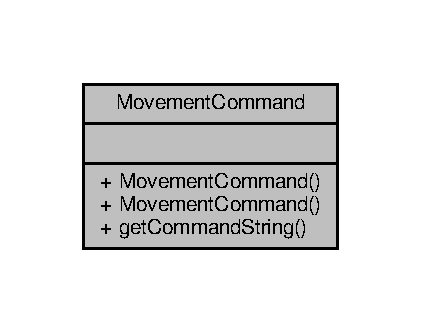
\includegraphics[width=202pt]{class_movement_command__coll__graph}
\end{center}
\end{figure}
\subsection*{Public Member Functions}
\begin{DoxyCompactItemize}
\item 
\hyperlink{class_movement_command_a23e01529fc28c324c05f71641e0fd0b5}{Movement\+Command} (uint8\+\_\+t channel, uint16\+\_\+t pulse\+Width, uint16\+\_\+t speed, uint16\+\_\+t time=0)
\begin{DoxyCompactList}\small\item\em Constructor. \end{DoxyCompactList}\item 
\hyperlink{class_movement_command_aa8b1442fc7cc7fcb50ff9a7d921d859b}{Movement\+Command} (std\+::string command)
\begin{DoxyCompactList}\small\item\em Constructor. \end{DoxyCompactList}\item 
std\+::string \hyperlink{class_movement_command_a93ad4b1cce1cb177c320e1b95170bc5c}{get\+Command\+String} ()
\begin{DoxyCompactList}\small\item\em Constructs the a message the controller understands given the class variables. \end{DoxyCompactList}\end{DoxyCompactItemize}


\subsection{Constructor \& Destructor Documentation}
\index{Movement\+Command@{Movement\+Command}!Movement\+Command@{Movement\+Command}}
\index{Movement\+Command@{Movement\+Command}!Movement\+Command@{Movement\+Command}}
\subsubsection[{\texorpdfstring{Movement\+Command(uint8\+\_\+t channel, uint16\+\_\+t pulse\+Width, uint16\+\_\+t speed, uint16\+\_\+t time=0)}{MovementCommand(uint8_t channel, uint16_t pulseWidth, uint16_t speed, uint16_t time=0)}}]{\setlength{\rightskip}{0pt plus 5cm}Movement\+Command\+::\+Movement\+Command (
\begin{DoxyParamCaption}
\item[{uint8\+\_\+t}]{channel, }
\item[{uint16\+\_\+t}]{pulse\+Width, }
\item[{uint16\+\_\+t}]{speed, }
\item[{uint16\+\_\+t}]{time = {\ttfamily 0}}
\end{DoxyParamCaption}
)\hspace{0.3cm}{\ttfamily [inline]}}\hypertarget{class_movement_command_a23e01529fc28c324c05f71641e0fd0b5}{}\label{class_movement_command_a23e01529fc28c324c05f71641e0fd0b5}


Constructor. 


\begin{DoxyParams}{Parameters}
{\em channel} & Channel the servo is connected to. \\
\hline
{\em pulse\+Width} & Pulse width in useq to move the servo to. \\
\hline
{\em speed} & Speed in useq/sec to move the servo in. \\
\hline
{\em time} & Time in miliseconds to move the servo in. \\
\hline
\end{DoxyParams}
\index{Movement\+Command@{Movement\+Command}!Movement\+Command@{Movement\+Command}}
\index{Movement\+Command@{Movement\+Command}!Movement\+Command@{Movement\+Command}}
\subsubsection[{\texorpdfstring{Movement\+Command(std\+::string command)}{MovementCommand(std::string command)}}]{\setlength{\rightskip}{0pt plus 5cm}Movement\+Command\+::\+Movement\+Command (
\begin{DoxyParamCaption}
\item[{std\+::string}]{command}
\end{DoxyParamCaption}
)\hspace{0.3cm}{\ttfamily [inline]}}\hypertarget{class_movement_command_aa8b1442fc7cc7fcb50ff9a7d921d859b}{}\label{class_movement_command_aa8b1442fc7cc7fcb50ff9a7d921d859b}


Constructor. 


\begin{DoxyParams}{Parameters}
{\em command} & Muliservo movement command. \\
\hline
\end{DoxyParams}


\subsection{Member Function Documentation}
\index{Movement\+Command@{Movement\+Command}!get\+Command\+String@{get\+Command\+String}}
\index{get\+Command\+String@{get\+Command\+String}!Movement\+Command@{Movement\+Command}}
\subsubsection[{\texorpdfstring{get\+Command\+String()}{getCommandString()}}]{\setlength{\rightskip}{0pt plus 5cm}std\+::string Movement\+Command\+::get\+Command\+String (
\begin{DoxyParamCaption}
{}
\end{DoxyParamCaption}
)\hspace{0.3cm}{\ttfamily [inline]}}\hypertarget{class_movement_command_a93ad4b1cce1cb177c320e1b95170bc5c}{}\label{class_movement_command_a93ad4b1cce1cb177c320e1b95170bc5c}


Constructs the a message the controller understands given the class variables. 

\begin{DoxyReturn}{Returns}
Returns a movement command for the controller. 
\end{DoxyReturn}


The documentation for this class was generated from the following file\+:\begin{DoxyCompactItemize}
\item 
\hyperlink{_movement_command_8hpp}{Movement\+Command.\+hpp}\end{DoxyCompactItemize}

\hypertarget{class_ros_communication}{}\section{Ros\+Communication Class Reference}
\label{class_ros_communication}\index{Ros\+Communication@{Ros\+Communication}}


{\ttfamily \#include $<$Ros\+Communication.\+hpp$>$}



Collaboration diagram for Ros\+Communication\+:
\nopagebreak
\begin{figure}[H]
\begin{center}
\leavevmode
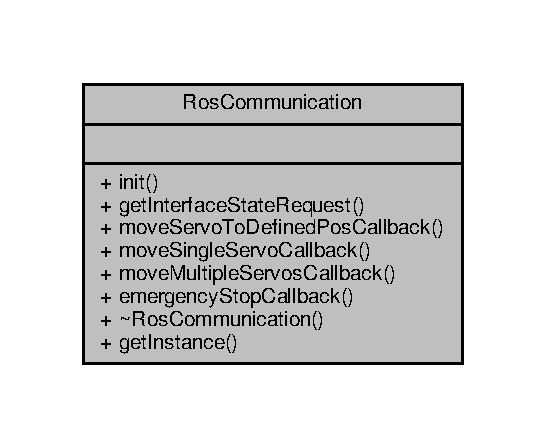
\includegraphics[width=262pt]{class_ros_communication__coll__graph}
\end{center}
\end{figure}
\subsection*{Public Member Functions}
\begin{DoxyCompactItemize}
\item 
bool \hyperlink{class_ros_communication_a42d1d1d9e470379bcbeec795ad27315c}{init} ()
\begin{DoxyCompactList}\small\item\em Initializes the ros communication. \end{DoxyCompactList}\item 
bool \hyperlink{class_ros_communication_a820758b87bc530aeda82eddb2d0550f9}{get\+Interface\+State\+Request} (Robotarm\+\_\+\+Interface\+::interface\+State\+Srv\+::\+Request \&req, Robotarm\+\_\+\+Interface\+::interface\+State\+Srv\+::\+Response \&res)
\begin{DoxyCompactList}\small\item\em Callback function for an interface state request. \end{DoxyCompactList}\item 
void \hyperlink{class_ros_communication_aa00bb61de93c1117510fd5625035d9ab}{move\+Servo\+To\+Defined\+Pos\+Callback} (const Robotarm\+\_\+\+Interface\+::move\+Servo\+Defined\+Msg \&msg)
\begin{DoxyCompactList}\small\item\em Handler when it receives an move\+Servo\+Defined\+Msg message. \end{DoxyCompactList}\item 
void \hyperlink{class_ros_communication_a946c6140b6e83b2568d51501aff4f228}{move\+Single\+Servo\+Callback} (const Robotarm\+\_\+\+Interface\+::move\+Single\+Servo\+Msg \&msg)
\begin{DoxyCompactList}\small\item\em Handler when it receives an move\+Single\+Servo\+Msg message. \end{DoxyCompactList}\item 
void \hyperlink{class_ros_communication_a7af24efba9be306ac689849574686ab4}{move\+Multiple\+Servos\+Callback} (const Robotarm\+\_\+\+Interface\+::move\+Multiple\+Servos\+Msg \&msg)
\begin{DoxyCompactList}\small\item\em Handler when it receives an move\+Multiple\+Servos\+Msg message. \end{DoxyCompactList}\item 
void \hyperlink{class_ros_communication_ab2d6174904dad1ce1a066f1d4a6c8fd8}{emergency\+Stop\+Callback} (const Robotarm\+\_\+\+Interface\+::emergency\+Stop\+Msg \&msg)
\begin{DoxyCompactList}\small\item\em Handler when it receives an emergency\+Stop\+Msg message. \end{DoxyCompactList}\item 
virtual \hyperlink{class_ros_communication_ab65e97f16b04e4a752d48f9f991c32a1}{$\sim$\+Ros\+Communication} ()
\end{DoxyCompactItemize}
\subsection*{Static Public Member Functions}
\begin{DoxyCompactItemize}
\item 
static \hyperlink{class_ros_communication}{Ros\+Communication} \& \hyperlink{class_ros_communication_a4e138754ad16b2a2743c28ff8afac919}{get\+Instance} ()
\begin{DoxyCompactList}\small\item\em Gets an \hyperlink{class_ros_communication}{Ros\+Communication} instance. \end{DoxyCompactList}\end{DoxyCompactItemize}


\subsection{Constructor \& Destructor Documentation}
\index{Ros\+Communication@{Ros\+Communication}!````~Ros\+Communication@{$\sim$\+Ros\+Communication}}
\index{````~Ros\+Communication@{$\sim$\+Ros\+Communication}!Ros\+Communication@{Ros\+Communication}}
\subsubsection[{\texorpdfstring{$\sim$\+Ros\+Communication()}{~RosCommunication()}}]{\setlength{\rightskip}{0pt plus 5cm}Ros\+Communication\+::$\sim$\+Ros\+Communication (
\begin{DoxyParamCaption}
{}
\end{DoxyParamCaption}
)\hspace{0.3cm}{\ttfamily [virtual]}}\hypertarget{class_ros_communication_ab65e97f16b04e4a752d48f9f991c32a1}{}\label{class_ros_communication_ab65e97f16b04e4a752d48f9f991c32a1}


\subsection{Member Function Documentation}
\index{Ros\+Communication@{Ros\+Communication}!emergency\+Stop\+Callback@{emergency\+Stop\+Callback}}
\index{emergency\+Stop\+Callback@{emergency\+Stop\+Callback}!Ros\+Communication@{Ros\+Communication}}
\subsubsection[{\texorpdfstring{emergency\+Stop\+Callback(const Robotarm\+\_\+\+Interface\+::emergency\+Stop\+Msg \&msg)}{emergencyStopCallback(const robotarminterface::emergencyStopMsg &msg)}}]{\setlength{\rightskip}{0pt plus 5cm}void Ros\+Communication\+::emergency\+Stop\+Callback (
\begin{DoxyParamCaption}
\item[{const Robotarm\+\_\+\+Interface\+::emergency\+Stop\+Msg \&}]{msg}
\end{DoxyParamCaption}
)}\hypertarget{class_ros_communication_ab2d6174904dad1ce1a066f1d4a6c8fd8}{}\label{class_ros_communication_ab2d6174904dad1ce1a066f1d4a6c8fd8}


Handler when it receives an emergency\+Stop\+Msg message. 


\begin{DoxyParams}{Parameters}
{\em msg} & Message type. \\
\hline
\end{DoxyParams}
\index{Ros\+Communication@{Ros\+Communication}!get\+Instance@{get\+Instance}}
\index{get\+Instance@{get\+Instance}!Ros\+Communication@{Ros\+Communication}}
\subsubsection[{\texorpdfstring{get\+Instance()}{getInstance()}}]{\setlength{\rightskip}{0pt plus 5cm}{\bf Ros\+Communication} \& Ros\+Communication\+::get\+Instance (
\begin{DoxyParamCaption}
{}
\end{DoxyParamCaption}
)\hspace{0.3cm}{\ttfamily [static]}}\hypertarget{class_ros_communication_a4e138754ad16b2a2743c28ff8afac919}{}\label{class_ros_communication_a4e138754ad16b2a2743c28ff8afac919}


Gets an \hyperlink{class_ros_communication}{Ros\+Communication} instance. 

\index{Ros\+Communication@{Ros\+Communication}!get\+Interface\+State\+Request@{get\+Interface\+State\+Request}}
\index{get\+Interface\+State\+Request@{get\+Interface\+State\+Request}!Ros\+Communication@{Ros\+Communication}}
\subsubsection[{\texorpdfstring{get\+Interface\+State\+Request(\+Robotarm\+\_\+\+Interface\+::interface\+State\+Srv\+::\+Request \&req, Robotarm\+\_\+\+Interface\+::interface\+State\+Srv\+::\+Response \&res)}{getInterfaceStateRequest(robotarminterface::interfaceStateSrv::Request &req, robotarminterface::interfaceStateSrv::Response &res)}}]{\setlength{\rightskip}{0pt plus 5cm}bool Ros\+Communication\+::get\+Interface\+State\+Request (
\begin{DoxyParamCaption}
\item[{Robotarm\+\_\+\+Interface\+::interface\+State\+Srv\+::\+Request \&}]{req, }
\item[{Robotarm\+\_\+\+Interface\+::interface\+State\+Srv\+::\+Response \&}]{res}
\end{DoxyParamCaption}
)}\hypertarget{class_ros_communication_a820758b87bc530aeda82eddb2d0550f9}{}\label{class_ros_communication_a820758b87bc530aeda82eddb2d0550f9}


Callback function for an interface state request. 


\begin{DoxyParams}{Parameters}
{\em req} & Request struct. \\
\hline
{\em res} & Response struct. \\
\hline
\end{DoxyParams}
\begin{DoxyReturn}{Returns}
Returns if ros can send the response back. 
\end{DoxyReturn}
\index{Ros\+Communication@{Ros\+Communication}!init@{init}}
\index{init@{init}!Ros\+Communication@{Ros\+Communication}}
\subsubsection[{\texorpdfstring{init()}{init()}}]{\setlength{\rightskip}{0pt plus 5cm}bool Ros\+Communication\+::init (
\begin{DoxyParamCaption}
{}
\end{DoxyParamCaption}
)}\hypertarget{class_ros_communication_a42d1d1d9e470379bcbeec795ad27315c}{}\label{class_ros_communication_a42d1d1d9e470379bcbeec795ad27315c}


Initializes the ros communication. 

\index{Ros\+Communication@{Ros\+Communication}!move\+Multiple\+Servos\+Callback@{move\+Multiple\+Servos\+Callback}}
\index{move\+Multiple\+Servos\+Callback@{move\+Multiple\+Servos\+Callback}!Ros\+Communication@{Ros\+Communication}}
\subsubsection[{\texorpdfstring{move\+Multiple\+Servos\+Callback(const Robotarm\+\_\+\+Interface\+::move\+Multiple\+Servos\+Msg \&msg)}{moveMultipleServosCallback(const robotarminterface::moveMultipleServosMsg &msg)}}]{\setlength{\rightskip}{0pt plus 5cm}void Ros\+Communication\+::move\+Multiple\+Servos\+Callback (
\begin{DoxyParamCaption}
\item[{const Robotarm\+\_\+\+Interface\+::move\+Multiple\+Servos\+Msg \&}]{msg}
\end{DoxyParamCaption}
)}\hypertarget{class_ros_communication_a7af24efba9be306ac689849574686ab4}{}\label{class_ros_communication_a7af24efba9be306ac689849574686ab4}


Handler when it receives an move\+Multiple\+Servos\+Msg message. 


\begin{DoxyParams}{Parameters}
{\em msg} & Message type. \\
\hline
\end{DoxyParams}
\index{Ros\+Communication@{Ros\+Communication}!move\+Servo\+To\+Defined\+Pos\+Callback@{move\+Servo\+To\+Defined\+Pos\+Callback}}
\index{move\+Servo\+To\+Defined\+Pos\+Callback@{move\+Servo\+To\+Defined\+Pos\+Callback}!Ros\+Communication@{Ros\+Communication}}
\subsubsection[{\texorpdfstring{move\+Servo\+To\+Defined\+Pos\+Callback(const Robotarm\+\_\+\+Interface\+::move\+Servo\+Defined\+Msg \&msg)}{moveServoToDefinedPosCallback(const robotarminterface::moveServoDefinedMsg &msg)}}]{\setlength{\rightskip}{0pt plus 5cm}void Ros\+Communication\+::move\+Servo\+To\+Defined\+Pos\+Callback (
\begin{DoxyParamCaption}
\item[{const Robotarm\+\_\+\+Interface\+::move\+Servo\+Defined\+Msg \&}]{msg}
\end{DoxyParamCaption}
)}\hypertarget{class_ros_communication_aa00bb61de93c1117510fd5625035d9ab}{}\label{class_ros_communication_aa00bb61de93c1117510fd5625035d9ab}


Handler when it receives an move\+Servo\+Defined\+Msg message. 


\begin{DoxyParams}{Parameters}
{\em msg} & Message type. \\
\hline
\end{DoxyParams}
\index{Ros\+Communication@{Ros\+Communication}!move\+Single\+Servo\+Callback@{move\+Single\+Servo\+Callback}}
\index{move\+Single\+Servo\+Callback@{move\+Single\+Servo\+Callback}!Ros\+Communication@{Ros\+Communication}}
\subsubsection[{\texorpdfstring{move\+Single\+Servo\+Callback(const Robotarm\+\_\+\+Interface\+::move\+Single\+Servo\+Msg \&msg)}{moveSingleServoCallback(const robotarminterface::moveSingleServoMsg &msg)}}]{\setlength{\rightskip}{0pt plus 5cm}void Ros\+Communication\+::move\+Single\+Servo\+Callback (
\begin{DoxyParamCaption}
\item[{const Robotarm\+\_\+\+Interface\+::move\+Single\+Servo\+Msg \&}]{msg}
\end{DoxyParamCaption}
)}\hypertarget{class_ros_communication_a946c6140b6e83b2568d51501aff4f228}{}\label{class_ros_communication_a946c6140b6e83b2568d51501aff4f228}


Handler when it receives an move\+Single\+Servo\+Msg message. 


\begin{DoxyParams}{Parameters}
{\em msg} & Message type. \\
\hline
\end{DoxyParams}


The documentation for this class was generated from the following files\+:\begin{DoxyCompactItemize}
\item 
\hyperlink{_ros_communication_8hpp}{Ros\+Communication.\+hpp}\item 
\hyperlink{_ros_communication_8cpp}{Ros\+Communication.\+cpp}\end{DoxyCompactItemize}

\hypertarget{class_serial_control}{}\section{Serial\+Control Class Reference}
\label{class_serial_control}\index{Serial\+Control@{Serial\+Control}}


{\ttfamily \#include $<$Serial\+Control.\+hpp$>$}



Collaboration diagram for Serial\+Control\+:
\nopagebreak
\begin{figure}[H]
\begin{center}
\leavevmode
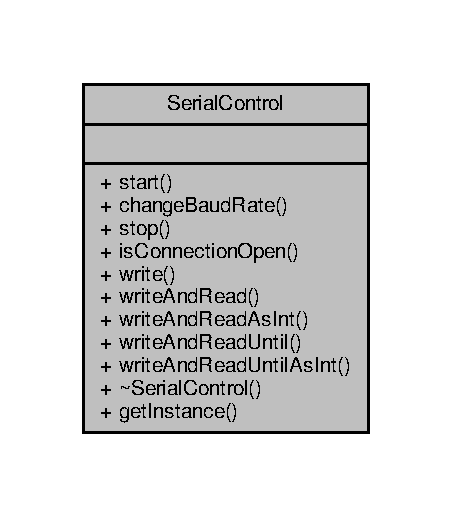
\includegraphics[width=217pt]{class_serial_control__coll__graph}
\end{center}
\end{figure}
\subsection*{Public Member Functions}
\begin{DoxyCompactItemize}
\item 
bool \hyperlink{class_serial_control_ab1a0d5fd054f401c2fe2b190476fb39a}{start} (const std\+::string \&port\+Name, uint32\+\_\+t baudrate)
\begin{DoxyCompactList}\small\item\em Starts the serial communication. \end{DoxyCompactList}\item 
void \hyperlink{class_serial_control_a3989d8baeb235db92234c48449e745de}{change\+Baud\+Rate} (const std\+::string \&port\+Name, uint32\+\_\+t baudrate)
\begin{DoxyCompactList}\small\item\em Changes the baudrate of the serial communication. \end{DoxyCompactList}\item 
void \hyperlink{class_serial_control_a023fb46d313a6c096641e085e86bf591}{stop} ()
\begin{DoxyCompactList}\small\item\em Stop and performs cleanup of the serial communication. \end{DoxyCompactList}\item 
bool \hyperlink{class_serial_control_a716c21c7b4abbb9361a7dc8ebd830324}{is\+Connection\+Open} ()
\begin{DoxyCompactList}\small\item\em Checks if a connection to a serial port is open. \end{DoxyCompactList}\item 
int \hyperlink{class_serial_control_a541d9b50b46fa00036921d05366ec078}{write} (const std\+::string \&message)
\begin{DoxyCompactList}\small\item\em Writes a string to the serial port. \end{DoxyCompactList}\item 
std\+::string \hyperlink{class_serial_control_a52a8a06063af9fb23d76e46d80692e32}{write\+And\+Read} (const std\+::string \&message, const size\+\_\+t response\+Size)
\begin{DoxyCompactList}\small\item\em Writes a message to the serial port and waits(blocking) for a response of a specific size. \end{DoxyCompactList}\item 
int \hyperlink{class_serial_control_a7632975d1edf2685411a4c7988f1941e}{write\+And\+Read\+As\+Int} (const std\+::string \&message, const size\+\_\+t response\+Size)
\begin{DoxyCompactList}\small\item\em Writes a message to the serial port and waits(blocking) for a response of a specific size. \end{DoxyCompactList}\item 
std\+::string \hyperlink{class_serial_control_a4e637cd5cf3bf8cc13d6b9852d0a891c}{write\+And\+Read\+Until} (const std\+::string \&message, const char until\+Char)
\begin{DoxyCompactList}\small\item\em Writes a message to the serial port and waits(blocking) for a response of a specific size. \end{DoxyCompactList}\item 
int \hyperlink{class_serial_control_aad283042dd26b2be94d78ac45c629751}{write\+And\+Read\+Until\+As\+Int} (const std\+::string \&message, const char until\+Char)
\begin{DoxyCompactList}\small\item\em Writes a message to the serial port and waits(blocking) for a response of a specific size. \end{DoxyCompactList}\item 
virtual \hyperlink{class_serial_control_a7a32ed21557bb9a0c92806d57435e5a3}{$\sim$\+Serial\+Control} ()
\end{DoxyCompactItemize}
\subsection*{Static Public Member Functions}
\begin{DoxyCompactItemize}
\item 
static \hyperlink{class_serial_control}{Serial\+Control} \& \hyperlink{class_serial_control_a5947ac36625386032cfce8deb07b65a9}{get\+Instance} ()
\begin{DoxyCompactList}\small\item\em Gets the a reference to a \hyperlink{class_serial_control}{Serial\+Control} instance. \end{DoxyCompactList}\end{DoxyCompactItemize}


\subsection{Constructor \& Destructor Documentation}
\index{Serial\+Control@{Serial\+Control}!````~Serial\+Control@{$\sim$\+Serial\+Control}}
\index{````~Serial\+Control@{$\sim$\+Serial\+Control}!Serial\+Control@{Serial\+Control}}
\subsubsection[{\texorpdfstring{$\sim$\+Serial\+Control()}{~SerialControl()}}]{\setlength{\rightskip}{0pt plus 5cm}Serial\+Control\+::$\sim$\+Serial\+Control (
\begin{DoxyParamCaption}
{}
\end{DoxyParamCaption}
)\hspace{0.3cm}{\ttfamily [virtual]}}\hypertarget{class_serial_control_a7a32ed21557bb9a0c92806d57435e5a3}{}\label{class_serial_control_a7a32ed21557bb9a0c92806d57435e5a3}


\subsection{Member Function Documentation}
\index{Serial\+Control@{Serial\+Control}!change\+Baud\+Rate@{change\+Baud\+Rate}}
\index{change\+Baud\+Rate@{change\+Baud\+Rate}!Serial\+Control@{Serial\+Control}}
\subsubsection[{\texorpdfstring{change\+Baud\+Rate(const std\+::string \&port\+Name, uint32\+\_\+t baudrate)}{changeBaudRate(const std::string &portName, uint32_t baudrate)}}]{\setlength{\rightskip}{0pt plus 5cm}void Serial\+Control\+::change\+Baud\+Rate (
\begin{DoxyParamCaption}
\item[{const std\+::string \&}]{port\+Name, }
\item[{uint32\+\_\+t}]{baudrate}
\end{DoxyParamCaption}
)}\hypertarget{class_serial_control_a3989d8baeb235db92234c48449e745de}{}\label{class_serial_control_a3989d8baeb235db92234c48449e745de}


Changes the baudrate of the serial communication. 


\begin{DoxyParams}{Parameters}
{\em port\+Name} & Port name on the pc the controller is connected to. \\
\hline
{\em baudrate} & Baudrate to run the serial communication on. \\
\hline
\end{DoxyParams}
\index{Serial\+Control@{Serial\+Control}!get\+Instance@{get\+Instance}}
\index{get\+Instance@{get\+Instance}!Serial\+Control@{Serial\+Control}}
\subsubsection[{\texorpdfstring{get\+Instance()}{getInstance()}}]{\setlength{\rightskip}{0pt plus 5cm}{\bf Serial\+Control} \& Serial\+Control\+::get\+Instance (
\begin{DoxyParamCaption}
{}
\end{DoxyParamCaption}
)\hspace{0.3cm}{\ttfamily [static]}}\hypertarget{class_serial_control_a5947ac36625386032cfce8deb07b65a9}{}\label{class_serial_control_a5947ac36625386032cfce8deb07b65a9}


Gets the a reference to a \hyperlink{class_serial_control}{Serial\+Control} instance. 

\index{Serial\+Control@{Serial\+Control}!is\+Connection\+Open@{is\+Connection\+Open}}
\index{is\+Connection\+Open@{is\+Connection\+Open}!Serial\+Control@{Serial\+Control}}
\subsubsection[{\texorpdfstring{is\+Connection\+Open()}{isConnectionOpen()}}]{\setlength{\rightskip}{0pt plus 5cm}bool Serial\+Control\+::is\+Connection\+Open (
\begin{DoxyParamCaption}
{}
\end{DoxyParamCaption}
)}\hypertarget{class_serial_control_a716c21c7b4abbb9361a7dc8ebd830324}{}\label{class_serial_control_a716c21c7b4abbb9361a7dc8ebd830324}


Checks if a connection to a serial port is open. 

\index{Serial\+Control@{Serial\+Control}!start@{start}}
\index{start@{start}!Serial\+Control@{Serial\+Control}}
\subsubsection[{\texorpdfstring{start(const std\+::string \&port\+Name, uint32\+\_\+t baudrate)}{start(const std::string &portName, uint32_t baudrate)}}]{\setlength{\rightskip}{0pt plus 5cm}bool Serial\+Control\+::start (
\begin{DoxyParamCaption}
\item[{const std\+::string \&}]{port\+Name, }
\item[{uint32\+\_\+t}]{baudrate}
\end{DoxyParamCaption}
)}\hypertarget{class_serial_control_ab1a0d5fd054f401c2fe2b190476fb39a}{}\label{class_serial_control_ab1a0d5fd054f401c2fe2b190476fb39a}


Starts the serial communication. 


\begin{DoxyParams}{Parameters}
{\em port\+Name} & Portname on the pc the controller is connected to. \\
\hline
{\em baudrate} & Baudrate to run the serial communication on. \\
\hline
\end{DoxyParams}
\begin{DoxyReturn}{Returns}
Returns true if the serial communication has succesfully been started. 
\end{DoxyReturn}
\index{Serial\+Control@{Serial\+Control}!stop@{stop}}
\index{stop@{stop}!Serial\+Control@{Serial\+Control}}
\subsubsection[{\texorpdfstring{stop()}{stop()}}]{\setlength{\rightskip}{0pt plus 5cm}void Serial\+Control\+::stop (
\begin{DoxyParamCaption}
{}
\end{DoxyParamCaption}
)}\hypertarget{class_serial_control_a023fb46d313a6c096641e085e86bf591}{}\label{class_serial_control_a023fb46d313a6c096641e085e86bf591}


Stop and performs cleanup of the serial communication. 

\index{Serial\+Control@{Serial\+Control}!write@{write}}
\index{write@{write}!Serial\+Control@{Serial\+Control}}
\subsubsection[{\texorpdfstring{write(const std\+::string \&message)}{write(const std::string &message)}}]{\setlength{\rightskip}{0pt plus 5cm}int Serial\+Control\+::write (
\begin{DoxyParamCaption}
\item[{const std\+::string \&}]{message}
\end{DoxyParamCaption}
)}\hypertarget{class_serial_control_a541d9b50b46fa00036921d05366ec078}{}\label{class_serial_control_a541d9b50b46fa00036921d05366ec078}


Writes a string to the serial port. 


\begin{DoxyParams}{Parameters}
{\em message} & String to write to the serial port. \\
\hline
\end{DoxyParams}
\begin{DoxyReturn}{Returns}
Returns the amount of bytes written. 
\end{DoxyReturn}
\index{Serial\+Control@{Serial\+Control}!write\+And\+Read@{write\+And\+Read}}
\index{write\+And\+Read@{write\+And\+Read}!Serial\+Control@{Serial\+Control}}
\subsubsection[{\texorpdfstring{write\+And\+Read(const std\+::string \&message, const size\+\_\+t response\+Size)}{writeAndRead(const std::string &message, const size_t responseSize)}}]{\setlength{\rightskip}{0pt plus 5cm}std\+::string Serial\+Control\+::write\+And\+Read (
\begin{DoxyParamCaption}
\item[{const std\+::string \&}]{message, }
\item[{const size\+\_\+t}]{response\+Size}
\end{DoxyParamCaption}
)}\hypertarget{class_serial_control_a52a8a06063af9fb23d76e46d80692e32}{}\label{class_serial_control_a52a8a06063af9fb23d76e46d80692e32}


Writes a message to the serial port and waits(blocking) for a response of a specific size. 


\begin{DoxyParams}{Parameters}
{\em message} & String to write to the serial port. \\
\hline
{\em response\+Size} & The size of the expected response (without \textquotesingle{}\textbackslash{}r\textquotesingle{} or \textquotesingle{}~\newline
\textquotesingle{}). \\
\hline
\end{DoxyParams}
\begin{DoxyReturn}{Returns}
Returns the response. 
\end{DoxyReturn}
\index{Serial\+Control@{Serial\+Control}!write\+And\+Read\+As\+Int@{write\+And\+Read\+As\+Int}}
\index{write\+And\+Read\+As\+Int@{write\+And\+Read\+As\+Int}!Serial\+Control@{Serial\+Control}}
\subsubsection[{\texorpdfstring{write\+And\+Read\+As\+Int(const std\+::string \&message, const size\+\_\+t response\+Size)}{writeAndReadAsInt(const std::string &message, const size_t responseSize)}}]{\setlength{\rightskip}{0pt plus 5cm}int Serial\+Control\+::write\+And\+Read\+As\+Int (
\begin{DoxyParamCaption}
\item[{const std\+::string \&}]{message, }
\item[{const size\+\_\+t}]{response\+Size}
\end{DoxyParamCaption}
)}\hypertarget{class_serial_control_a7632975d1edf2685411a4c7988f1941e}{}\label{class_serial_control_a7632975d1edf2685411a4c7988f1941e}


Writes a message to the serial port and waits(blocking) for a response of a specific size. 


\begin{DoxyParams}{Parameters}
{\em message} & String to write to the serial port. \\
\hline
{\em response\+Size} & The size of the expected response (without \textquotesingle{}\textbackslash{}r\textquotesingle{} or \textquotesingle{}~\newline
\textquotesingle{}). \\
\hline
\end{DoxyParams}
\begin{DoxyReturn}{Returns}
Returns the response as int. 
\end{DoxyReturn}
\index{Serial\+Control@{Serial\+Control}!write\+And\+Read\+Until@{write\+And\+Read\+Until}}
\index{write\+And\+Read\+Until@{write\+And\+Read\+Until}!Serial\+Control@{Serial\+Control}}
\subsubsection[{\texorpdfstring{write\+And\+Read\+Until(const std\+::string \&message, const char until\+Char)}{writeAndReadUntil(const std::string &message, const char untilChar)}}]{\setlength{\rightskip}{0pt plus 5cm}std\+::string Serial\+Control\+::write\+And\+Read\+Until (
\begin{DoxyParamCaption}
\item[{const std\+::string \&}]{message, }
\item[{const char}]{until\+Char}
\end{DoxyParamCaption}
)}\hypertarget{class_serial_control_a4e637cd5cf3bf8cc13d6b9852d0a891c}{}\label{class_serial_control_a4e637cd5cf3bf8cc13d6b9852d0a891c}


Writes a message to the serial port and waits(blocking) for a response of a specific size. 


\begin{DoxyParams}{Parameters}
{\em message} & String to write to the serial port. \\
\hline
{\em until\+Char} & Reads from string until it reads this character. \\
\hline
\end{DoxyParams}
\begin{DoxyReturn}{Returns}
Returns the response. 
\end{DoxyReturn}
\index{Serial\+Control@{Serial\+Control}!write\+And\+Read\+Until\+As\+Int@{write\+And\+Read\+Until\+As\+Int}}
\index{write\+And\+Read\+Until\+As\+Int@{write\+And\+Read\+Until\+As\+Int}!Serial\+Control@{Serial\+Control}}
\subsubsection[{\texorpdfstring{write\+And\+Read\+Until\+As\+Int(const std\+::string \&message, const char until\+Char)}{writeAndReadUntilAsInt(const std::string &message, const char untilChar)}}]{\setlength{\rightskip}{0pt plus 5cm}int Serial\+Control\+::write\+And\+Read\+Until\+As\+Int (
\begin{DoxyParamCaption}
\item[{const std\+::string \&}]{message, }
\item[{const char}]{until\+Char}
\end{DoxyParamCaption}
)}\hypertarget{class_serial_control_aad283042dd26b2be94d78ac45c629751}{}\label{class_serial_control_aad283042dd26b2be94d78ac45c629751}


Writes a message to the serial port and waits(blocking) for a response of a specific size. 


\begin{DoxyParams}{Parameters}
{\em message} & String to write to the serial port. \\
\hline
{\em until\+Char} & Reads from string until it reads this character. \\
\hline
\end{DoxyParams}
\begin{DoxyReturn}{Returns}
Returns the response as int. 
\end{DoxyReturn}


The documentation for this class was generated from the following files\+:\begin{DoxyCompactItemize}
\item 
\hyperlink{_serial_control_8hpp}{Serial\+Control.\+hpp}\item 
\hyperlink{_serial_control_8cpp}{Serial\+Control.\+cpp}\end{DoxyCompactItemize}

\hypertarget{class_servo}{}\section{Servo Class Reference}
\label{class_servo}\index{Servo@{Servo}}


{\ttfamily \#include $<$Servo.\+hpp$>$}



Collaboration diagram for Servo\+:
\nopagebreak
\begin{figure}[H]
\begin{center}
\leavevmode
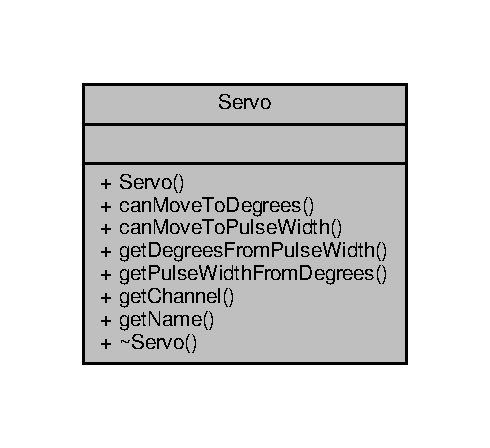
\includegraphics[width=235pt]{class_servo__coll__graph}
\end{center}
\end{figure}
\subsection*{Public Member Functions}
\begin{DoxyCompactItemize}
\item 
\hyperlink{class_servo_a584bf7fe3e64be597d73b999ef188943}{Servo} (uint8\+\_\+t channel, std\+::string name, int16\+\_\+t min\+Rotation, int16\+\_\+t max\+Rotation, uint16\+\_\+t min\+Pulse\+Width, uint16\+\_\+t max\+Pulse\+Width, int16\+\_\+t min\+Safe\+Rotation, int16\+\_\+t max\+Safe\+Rotation, double max\+Speed, bool inverted=false)
\begin{DoxyCompactList}\small\item\em Constructor. \end{DoxyCompactList}\item 
bool \hyperlink{class_servo_a46bad3775a3ee6942a3b0be5dea6756c}{can\+Move\+To\+Degrees} (int16\+\_\+t degrees) const 
\begin{DoxyCompactList}\small\item\em Checks if this servo can move to a specific rotation. \end{DoxyCompactList}\item 
bool \hyperlink{class_servo_afeecdc6812c2714b1e20e47bea6eacc5}{can\+Move\+To\+Pulse\+Width} (uint16\+\_\+t pulse\+Width) const 
\begin{DoxyCompactList}\small\item\em Checks if the servo can move to a specific pulsewidth. \end{DoxyCompactList}\item 
int16\+\_\+t \hyperlink{class_servo_a141a8ac9632728e2d09403f12b68d1b6}{get\+Degrees\+From\+Pulse\+Width} (uint16\+\_\+t pulse\+Width) const 
\begin{DoxyCompactList}\small\item\em Converts a pulse width to degrees. \end{DoxyCompactList}\item 
uint16\+\_\+t \hyperlink{class_servo_a0966d45b0fb13881a1f5b62ec2e59f10}{get\+Pulse\+Width\+From\+Degrees} (int16\+\_\+t degrees) const 
\begin{DoxyCompactList}\small\item\em Converts a rotation in degrees to a pulse width. \end{DoxyCompactList}\item 
uint8\+\_\+t \hyperlink{class_servo_addd646c6e9c088000cd7421679823661}{get\+Channel} () const 
\begin{DoxyCompactList}\small\item\em Gets the servo\textquotesingle{}s channel. \end{DoxyCompactList}\item 
const std\+::string \& \hyperlink{class_servo_a561a048a0de1fa3ac59c946186177f29}{get\+Name} () const 
\begin{DoxyCompactList}\small\item\em Gets the servo\textquotesingle{}s name. \end{DoxyCompactList}\item 
virtual \hyperlink{class_servo_a5dbcb967390f530c81c9246472e2d4c7}{$\sim$\+Servo} ()
\end{DoxyCompactItemize}


\subsection{Constructor \& Destructor Documentation}
\index{Servo@{Servo}!Servo@{Servo}}
\index{Servo@{Servo}!Servo@{Servo}}
\subsubsection[{\texorpdfstring{Servo(uint8\+\_\+t channel, std\+::string name, int16\+\_\+t min\+Rotation, int16\+\_\+t max\+Rotation, uint16\+\_\+t min\+Pulse\+Width, uint16\+\_\+t max\+Pulse\+Width, int16\+\_\+t min\+Safe\+Rotation, int16\+\_\+t max\+Safe\+Rotation, double max\+Speed, bool inverted=false)}{Servo(uint8_t channel, std::string name, int16_t minRotation, int16_t maxRotation, uint16_t minPulseWidth, uint16_t maxPulseWidth, int16_t minSafeRotation, int16_t maxSafeRotation, double maxSpeed, bool inverted=false)}}]{\setlength{\rightskip}{0pt plus 5cm}Servo\+::\+Servo (
\begin{DoxyParamCaption}
\item[{uint8\+\_\+t}]{channel, }
\item[{std\+::string}]{name, }
\item[{int16\+\_\+t}]{min\+Rotation, }
\item[{int16\+\_\+t}]{max\+Rotation, }
\item[{uint16\+\_\+t}]{min\+Pulse\+Width, }
\item[{uint16\+\_\+t}]{max\+Pulse\+Width, }
\item[{int16\+\_\+t}]{min\+Safe\+Rotation, }
\item[{int16\+\_\+t}]{max\+Safe\+Rotation, }
\item[{double}]{max\+Speed, }
\item[{bool}]{inverted = {\ttfamily false}}
\end{DoxyParamCaption}
)\hspace{0.3cm}{\ttfamily [inline]}}\hypertarget{class_servo_a584bf7fe3e64be597d73b999ef188943}{}\label{class_servo_a584bf7fe3e64be597d73b999ef188943}


Constructor. 


\begin{DoxyParams}{Parameters}
{\em channel} & Channel the servo is connected too. \\
\hline
{\em name} & Name of the servo. \\
\hline
{\em min\+Rotation} & Minimum rotation in degrees the servo can rotate to. \\
\hline
{\em max\+Rotation} & Maximum rotation in degrees the servo can rotate to. \\
\hline
{\em min\+Pulse\+Width} & Minimum pulse width in useq the servo can rotate to. \\
\hline
{\em max\+Pulse\+Width} & Maximum pulse width in useq the servo can rotate to. \\
\hline
{\em min\+Safe\+Rotation} & Minimum rotation in degrees it is safe to rotate the servo in. \\
\hline
{\em max\+Safe\+Rotation} & Maximum rotation in degrees it is safe to rotate the servo in. \\
\hline
{\em max\+Speed} & Speed in useq per 60 degrees. \\
\hline
{\em inverted} & If the servo is reversed. \\
\hline
\end{DoxyParams}
\index{Servo@{Servo}!````~Servo@{$\sim$\+Servo}}
\index{````~Servo@{$\sim$\+Servo}!Servo@{Servo}}
\subsubsection[{\texorpdfstring{$\sim$\+Servo()}{~Servo()}}]{\setlength{\rightskip}{0pt plus 5cm}virtual Servo\+::$\sim$\+Servo (
\begin{DoxyParamCaption}
{}
\end{DoxyParamCaption}
)\hspace{0.3cm}{\ttfamily [inline]}, {\ttfamily [virtual]}}\hypertarget{class_servo_a5dbcb967390f530c81c9246472e2d4c7}{}\label{class_servo_a5dbcb967390f530c81c9246472e2d4c7}


\subsection{Member Function Documentation}
\index{Servo@{Servo}!can\+Move\+To\+Degrees@{can\+Move\+To\+Degrees}}
\index{can\+Move\+To\+Degrees@{can\+Move\+To\+Degrees}!Servo@{Servo}}
\subsubsection[{\texorpdfstring{can\+Move\+To\+Degrees(int16\+\_\+t degrees) const }{canMoveToDegrees(int16_t degrees) const }}]{\setlength{\rightskip}{0pt plus 5cm}bool Servo\+::can\+Move\+To\+Degrees (
\begin{DoxyParamCaption}
\item[{int16\+\_\+t}]{degrees}
\end{DoxyParamCaption}
) const\hspace{0.3cm}{\ttfamily [inline]}}\hypertarget{class_servo_a46bad3775a3ee6942a3b0be5dea6756c}{}\label{class_servo_a46bad3775a3ee6942a3b0be5dea6756c}


Checks if this servo can move to a specific rotation. 


\begin{DoxyParams}{Parameters}
{\em degrees} & Rotation in degrees to check. \\
\hline
\end{DoxyParams}
\begin{DoxyReturn}{Returns}
True if possible. 
\end{DoxyReturn}
\index{Servo@{Servo}!can\+Move\+To\+Pulse\+Width@{can\+Move\+To\+Pulse\+Width}}
\index{can\+Move\+To\+Pulse\+Width@{can\+Move\+To\+Pulse\+Width}!Servo@{Servo}}
\subsubsection[{\texorpdfstring{can\+Move\+To\+Pulse\+Width(uint16\+\_\+t pulse\+Width) const }{canMoveToPulseWidth(uint16_t pulseWidth) const }}]{\setlength{\rightskip}{0pt plus 5cm}bool Servo\+::can\+Move\+To\+Pulse\+Width (
\begin{DoxyParamCaption}
\item[{uint16\+\_\+t}]{pulse\+Width}
\end{DoxyParamCaption}
) const\hspace{0.3cm}{\ttfamily [inline]}}\hypertarget{class_servo_afeecdc6812c2714b1e20e47bea6eacc5}{}\label{class_servo_afeecdc6812c2714b1e20e47bea6eacc5}


Checks if the servo can move to a specific pulsewidth. 


\begin{DoxyParams}{Parameters}
{\em pulse\+Width} & Pulse width in usec. \\
\hline
\end{DoxyParams}
\begin{DoxyReturn}{Returns}
True if possible. 
\end{DoxyReturn}
\index{Servo@{Servo}!get\+Channel@{get\+Channel}}
\index{get\+Channel@{get\+Channel}!Servo@{Servo}}
\subsubsection[{\texorpdfstring{get\+Channel() const }{getChannel() const }}]{\setlength{\rightskip}{0pt plus 5cm}uint8\+\_\+t Servo\+::get\+Channel (
\begin{DoxyParamCaption}
{}
\end{DoxyParamCaption}
) const\hspace{0.3cm}{\ttfamily [inline]}}\hypertarget{class_servo_addd646c6e9c088000cd7421679823661}{}\label{class_servo_addd646c6e9c088000cd7421679823661}


Gets the servo\textquotesingle{}s channel. 

\begin{DoxyReturn}{Returns}
Returns the servo\textquotesingle{}s channel. 
\end{DoxyReturn}
\index{Servo@{Servo}!get\+Degrees\+From\+Pulse\+Width@{get\+Degrees\+From\+Pulse\+Width}}
\index{get\+Degrees\+From\+Pulse\+Width@{get\+Degrees\+From\+Pulse\+Width}!Servo@{Servo}}
\subsubsection[{\texorpdfstring{get\+Degrees\+From\+Pulse\+Width(uint16\+\_\+t pulse\+Width) const }{getDegreesFromPulseWidth(uint16_t pulseWidth) const }}]{\setlength{\rightskip}{0pt plus 5cm}int16\+\_\+t Servo\+::get\+Degrees\+From\+Pulse\+Width (
\begin{DoxyParamCaption}
\item[{uint16\+\_\+t}]{pulse\+Width}
\end{DoxyParamCaption}
) const\hspace{0.3cm}{\ttfamily [inline]}}\hypertarget{class_servo_a141a8ac9632728e2d09403f12b68d1b6}{}\label{class_servo_a141a8ac9632728e2d09403f12b68d1b6}


Converts a pulse width to degrees. 

Returns 0 if the conversion is not possible. 
\begin{DoxyParams}{Parameters}
{\em pulse\+Width} & Pulse width in usec. \\
\hline
\end{DoxyParams}
\begin{DoxyReturn}{Returns}
Returns the rotation in degrees corresponding that pulse width. 
\end{DoxyReturn}
\index{Servo@{Servo}!get\+Name@{get\+Name}}
\index{get\+Name@{get\+Name}!Servo@{Servo}}
\subsubsection[{\texorpdfstring{get\+Name() const }{getName() const }}]{\setlength{\rightskip}{0pt plus 5cm}const std\+::string\& Servo\+::get\+Name (
\begin{DoxyParamCaption}
{}
\end{DoxyParamCaption}
) const\hspace{0.3cm}{\ttfamily [inline]}}\hypertarget{class_servo_a561a048a0de1fa3ac59c946186177f29}{}\label{class_servo_a561a048a0de1fa3ac59c946186177f29}


Gets the servo\textquotesingle{}s name. 

\begin{DoxyReturn}{Returns}
Returns the servo\textquotesingle{}s name. 
\end{DoxyReturn}
\index{Servo@{Servo}!get\+Pulse\+Width\+From\+Degrees@{get\+Pulse\+Width\+From\+Degrees}}
\index{get\+Pulse\+Width\+From\+Degrees@{get\+Pulse\+Width\+From\+Degrees}!Servo@{Servo}}
\subsubsection[{\texorpdfstring{get\+Pulse\+Width\+From\+Degrees(int16\+\_\+t degrees) const }{getPulseWidthFromDegrees(int16_t degrees) const }}]{\setlength{\rightskip}{0pt plus 5cm}uint16\+\_\+t Servo\+::get\+Pulse\+Width\+From\+Degrees (
\begin{DoxyParamCaption}
\item[{int16\+\_\+t}]{degrees}
\end{DoxyParamCaption}
) const\hspace{0.3cm}{\ttfamily [inline]}}\hypertarget{class_servo_a0966d45b0fb13881a1f5b62ec2e59f10}{}\label{class_servo_a0966d45b0fb13881a1f5b62ec2e59f10}


Converts a rotation in degrees to a pulse width. 

Returns 0 if the conversion is not possible. 
\begin{DoxyParams}{Parameters}
{\em degrees} & Rotation in degrees to convert. \\
\hline
\end{DoxyParams}
\begin{DoxyReturn}{Returns}
Returns the pulse width in useq corresponding that rotation. 
\end{DoxyReturn}


The documentation for this class was generated from the following file\+:\begin{DoxyCompactItemize}
\item 
\hyperlink{_servo_8hpp}{Servo.\+hpp}\end{DoxyCompactItemize}

\hypertarget{class_smart_queue}{}\section{Smart\+Queue$<$ T $>$ Class Template Reference}
\label{class_smart_queue}\index{Smart\+Queue$<$ T $>$@{Smart\+Queue$<$ T $>$}}


{\ttfamily \#include $<$Smart\+Queue.\+hpp$>$}



Collaboration diagram for Smart\+Queue$<$ T $>$\+:
\nopagebreak
\begin{figure}[H]
\begin{center}
\leavevmode
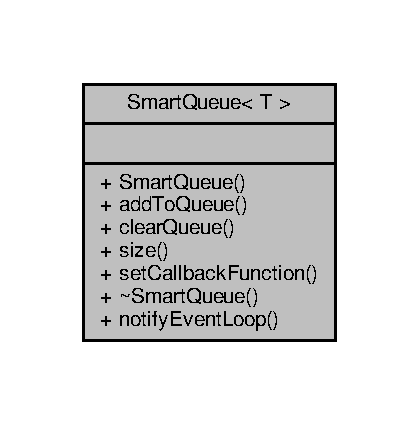
\includegraphics[width=201pt]{class_smart_queue__coll__graph}
\end{center}
\end{figure}
\subsection*{Public Member Functions}
\begin{DoxyCompactItemize}
\item 
\hyperlink{class_smart_queue_a12e3ef3a3d1ed0062f28fb6ae43c8acf}{Smart\+Queue} ()
\begin{DoxyCompactList}\small\item\em Constructor. \end{DoxyCompactList}\item 
void \hyperlink{class_smart_queue_a896d489b174bb960afd9bab1ee246ac6}{add\+To\+Queue} (const std\+::shared\+\_\+ptr$<$ T $>$ a\+Event)
\begin{DoxyCompactList}\small\item\em Adds an instance to the queue. \end{DoxyCompactList}\item 
void \hyperlink{class_smart_queue_a0d5f30e34e453d08103a587388a67617}{clear\+Queue} ()
\begin{DoxyCompactList}\small\item\em Removes all pending elements from the queue. \end{DoxyCompactList}\item 
size\+\_\+t \hyperlink{class_smart_queue_a05ad94528926d623d8fcb8da042cd889}{size} ()
\begin{DoxyCompactList}\small\item\em Returns the amount of elements in the queue. \end{DoxyCompactList}\item 
void \hyperlink{class_smart_queue_ac7f9a4d34bc09b2d2ea66aa91f418564}{set\+Callback\+Function} (std\+::function$<$ void(std\+::shared\+\_\+ptr$<$ T $>$)$>$ a)
\begin{DoxyCompactList}\small\item\em Sets a function to call when an element leaves the queue. \end{DoxyCompactList}\item 
virtual \hyperlink{class_smart_queue_aa1de2438e3776b873787e915f7adf356}{$\sim$\+Smart\+Queue} ()
\item 
void \hyperlink{class_smart_queue_ac8d665c15c424974a7eae42ba1cc3ad9}{notify\+Event\+Loop} ()
\begin{DoxyCompactList}\small\item\em Function that signals the event loop there is some work to do. \end{DoxyCompactList}\end{DoxyCompactItemize}


\subsection{Constructor \& Destructor Documentation}
\index{Smart\+Queue@{Smart\+Queue}!Smart\+Queue@{Smart\+Queue}}
\index{Smart\+Queue@{Smart\+Queue}!Smart\+Queue@{Smart\+Queue}}
\subsubsection[{\texorpdfstring{Smart\+Queue()}{SmartQueue()}}]{\setlength{\rightskip}{0pt plus 5cm}template$<$class T$>$ {\bf Smart\+Queue}$<$ T $>$\+::{\bf Smart\+Queue} (
\begin{DoxyParamCaption}
{}
\end{DoxyParamCaption}
)\hspace{0.3cm}{\ttfamily [inline]}}\hypertarget{class_smart_queue_a12e3ef3a3d1ed0062f28fb6ae43c8acf}{}\label{class_smart_queue_a12e3ef3a3d1ed0062f28fb6ae43c8acf}


Constructor. 

\index{Smart\+Queue@{Smart\+Queue}!````~Smart\+Queue@{$\sim$\+Smart\+Queue}}
\index{````~Smart\+Queue@{$\sim$\+Smart\+Queue}!Smart\+Queue@{Smart\+Queue}}
\subsubsection[{\texorpdfstring{$\sim$\+Smart\+Queue()}{~SmartQueue()}}]{\setlength{\rightskip}{0pt plus 5cm}template$<$class T$>$ virtual {\bf Smart\+Queue}$<$ T $>$\+::$\sim${\bf Smart\+Queue} (
\begin{DoxyParamCaption}
{}
\end{DoxyParamCaption}
)\hspace{0.3cm}{\ttfamily [inline]}, {\ttfamily [virtual]}}\hypertarget{class_smart_queue_aa1de2438e3776b873787e915f7adf356}{}\label{class_smart_queue_aa1de2438e3776b873787e915f7adf356}


\subsection{Member Function Documentation}
\index{Smart\+Queue@{Smart\+Queue}!add\+To\+Queue@{add\+To\+Queue}}
\index{add\+To\+Queue@{add\+To\+Queue}!Smart\+Queue@{Smart\+Queue}}
\subsubsection[{\texorpdfstring{add\+To\+Queue(const std\+::shared\+\_\+ptr$<$ T $>$ a\+Event)}{addToQueue(const std::shared_ptr< T > aEvent)}}]{\setlength{\rightskip}{0pt plus 5cm}template$<$class T$>$ void {\bf Smart\+Queue}$<$ T $>$\+::add\+To\+Queue (
\begin{DoxyParamCaption}
\item[{const std\+::shared\+\_\+ptr$<$ T $>$}]{a\+Event}
\end{DoxyParamCaption}
)\hspace{0.3cm}{\ttfamily [inline]}}\hypertarget{class_smart_queue_a896d489b174bb960afd9bab1ee246ac6}{}\label{class_smart_queue_a896d489b174bb960afd9bab1ee246ac6}


Adds an instance to the queue. 


\begin{DoxyParams}{Parameters}
{\em a\+Event} & Sharedpointer with the class instance. \\
\hline
\end{DoxyParams}
\index{Smart\+Queue@{Smart\+Queue}!clear\+Queue@{clear\+Queue}}
\index{clear\+Queue@{clear\+Queue}!Smart\+Queue@{Smart\+Queue}}
\subsubsection[{\texorpdfstring{clear\+Queue()}{clearQueue()}}]{\setlength{\rightskip}{0pt plus 5cm}template$<$class T$>$ void {\bf Smart\+Queue}$<$ T $>$\+::clear\+Queue (
\begin{DoxyParamCaption}
{}
\end{DoxyParamCaption}
)\hspace{0.3cm}{\ttfamily [inline]}}\hypertarget{class_smart_queue_a0d5f30e34e453d08103a587388a67617}{}\label{class_smart_queue_a0d5f30e34e453d08103a587388a67617}


Removes all pending elements from the queue. 

\index{Smart\+Queue@{Smart\+Queue}!notify\+Event\+Loop@{notify\+Event\+Loop}}
\index{notify\+Event\+Loop@{notify\+Event\+Loop}!Smart\+Queue@{Smart\+Queue}}
\subsubsection[{\texorpdfstring{notify\+Event\+Loop()}{notifyEventLoop()}}]{\setlength{\rightskip}{0pt plus 5cm}template$<$class T$>$ void {\bf Smart\+Queue}$<$ T $>$\+::notify\+Event\+Loop (
\begin{DoxyParamCaption}
{}
\end{DoxyParamCaption}
)\hspace{0.3cm}{\ttfamily [inline]}}\hypertarget{class_smart_queue_ac8d665c15c424974a7eae42ba1cc3ad9}{}\label{class_smart_queue_ac8d665c15c424974a7eae42ba1cc3ad9}


Function that signals the event loop there is some work to do. 

\index{Smart\+Queue@{Smart\+Queue}!set\+Callback\+Function@{set\+Callback\+Function}}
\index{set\+Callback\+Function@{set\+Callback\+Function}!Smart\+Queue@{Smart\+Queue}}
\subsubsection[{\texorpdfstring{set\+Callback\+Function(std\+::function$<$ void(std\+::shared\+\_\+ptr$<$ T $>$)$>$ a)}{setCallbackFunction(std::function< void(std::shared_ptr< T >)> a)}}]{\setlength{\rightskip}{0pt plus 5cm}template$<$class T$>$ void {\bf Smart\+Queue}$<$ T $>$\+::set\+Callback\+Function (
\begin{DoxyParamCaption}
\item[{std\+::function$<$ void(std\+::shared\+\_\+ptr$<$ T $>$)$>$}]{a}
\end{DoxyParamCaption}
)\hspace{0.3cm}{\ttfamily [inline]}}\hypertarget{class_smart_queue_ac7f9a4d34bc09b2d2ea66aa91f418564}{}\label{class_smart_queue_ac7f9a4d34bc09b2d2ea66aa91f418564}


Sets a function to call when an element leaves the queue. 


\begin{DoxyParams}{Parameters}
{\em a} & A function matching the template. \\
\hline
\end{DoxyParams}
\index{Smart\+Queue@{Smart\+Queue}!size@{size}}
\index{size@{size}!Smart\+Queue@{Smart\+Queue}}
\subsubsection[{\texorpdfstring{size()}{size()}}]{\setlength{\rightskip}{0pt plus 5cm}template$<$class T$>$ size\+\_\+t {\bf Smart\+Queue}$<$ T $>$\+::size (
\begin{DoxyParamCaption}
{}
\end{DoxyParamCaption}
)\hspace{0.3cm}{\ttfamily [inline]}}\hypertarget{class_smart_queue_a05ad94528926d623d8fcb8da042cd889}{}\label{class_smart_queue_a05ad94528926d623d8fcb8da042cd889}


Returns the amount of elements in the queue. 



The documentation for this class was generated from the following file\+:\begin{DoxyCompactItemize}
\item 
\hyperlink{_smart_queue_8hpp}{Smart\+Queue.\+hpp}\end{DoxyCompactItemize}

\chapter{File Documentation}
\hypertarget{main_8cpp}{}\section{main.\+cpp File Reference}
\label{main_8cpp}\index{main.\+cpp@{main.\+cpp}}
{\ttfamily \#include \char`\"{}ros/ros.\+h\char`\"{}}\\*
{\ttfamily \#include \char`\"{}Ros\+Communication.\+hpp\char`\"{}}\\*
{\ttfamily \#include \char`\"{}Motion\+Control.\+hpp\char`\"{}}\\*
{\ttfamily \#include \char`\"{}Serial\+Control.\+hpp\char`\"{}}\\*
{\ttfamily \#include $<$iostream$>$}\\*
{\ttfamily \#include $<$thread$>$}\\*
Include dependency graph for main.\+cpp\+:
\nopagebreak
\begin{figure}[H]
\begin{center}
\leavevmode
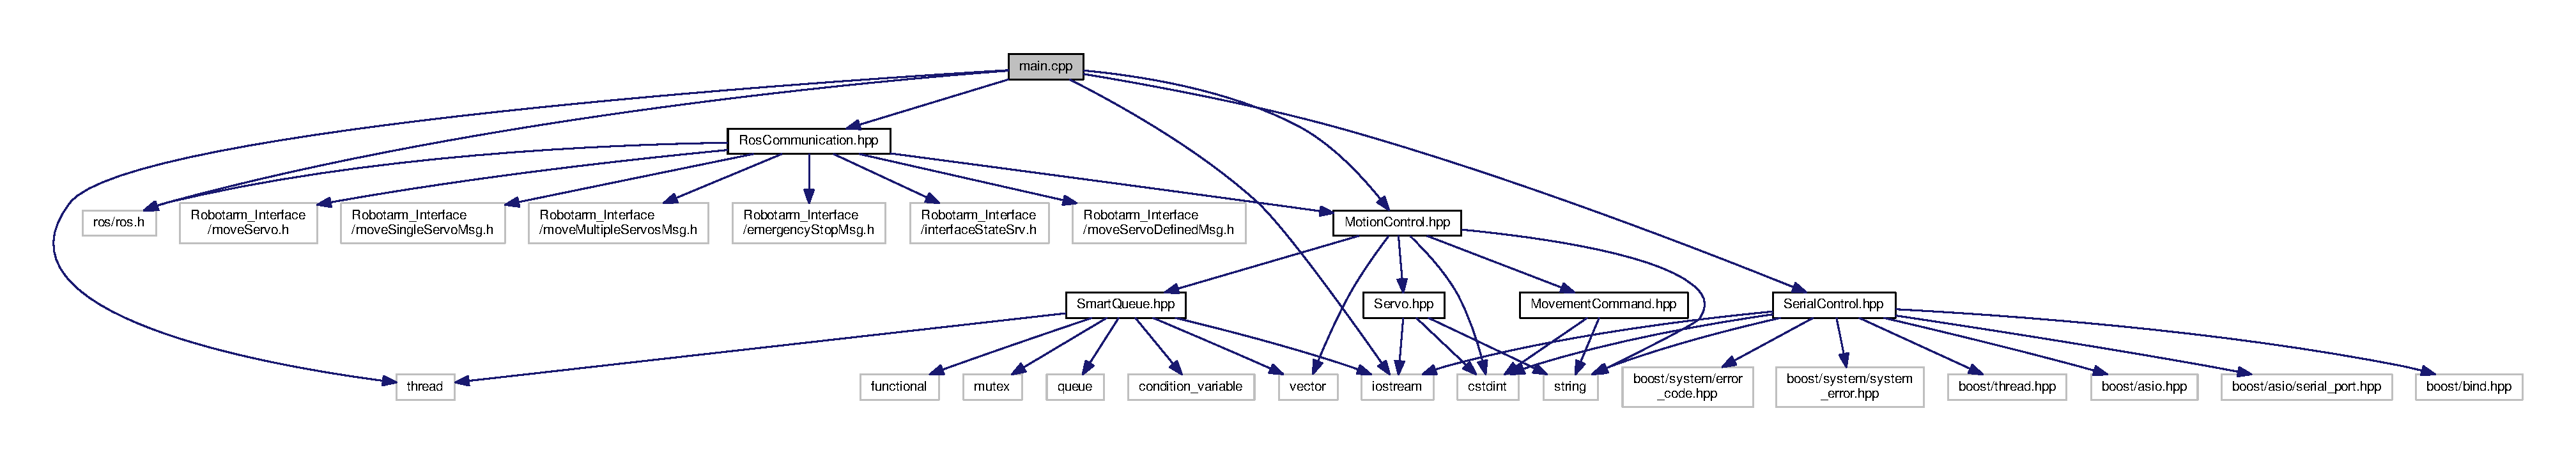
\includegraphics[width=350pt]{main_8cpp__incl}
\end{center}
\end{figure}
\subsection*{Functions}
\begin{DoxyCompactItemize}
\item 
int \hyperlink{main_8cpp_a0ddf1224851353fc92bfbff6f499fa97}{main} (int argc, char $\ast$argv\mbox{[}$\,$\mbox{]})
\end{DoxyCompactItemize}


\subsection{Function Documentation}
\index{main.\+cpp@{main.\+cpp}!main@{main}}
\index{main@{main}!main.\+cpp@{main.\+cpp}}
\subsubsection[{\texorpdfstring{main(int argc, char $\ast$argv[])}{main(int argc, char *argv[])}}]{\setlength{\rightskip}{0pt plus 5cm}int main (
\begin{DoxyParamCaption}
\item[{int}]{argc, }
\item[{char $\ast$}]{argv\mbox{[}$\,$\mbox{]}}
\end{DoxyParamCaption}
)}\hypertarget{main_8cpp_a0ddf1224851353fc92bfbff6f499fa97}{}\label{main_8cpp_a0ddf1224851353fc92bfbff6f499fa97}

\hypertarget{_motion_control_8cpp}{}\section{Motion\+Control.\+cpp File Reference}
\label{_motion_control_8cpp}\index{Motion\+Control.\+cpp@{Motion\+Control.\+cpp}}
{\ttfamily \#include \char`\"{}Motion\+Control.\+hpp\char`\"{}}\\*
{\ttfamily \#include \char`\"{}Serial\+Control.\+hpp\char`\"{}}\\*
{\ttfamily \#include $<$thread$>$}\\*
Include dependency graph for Motion\+Control.\+cpp\+:
\nopagebreak
\begin{figure}[H]
\begin{center}
\leavevmode
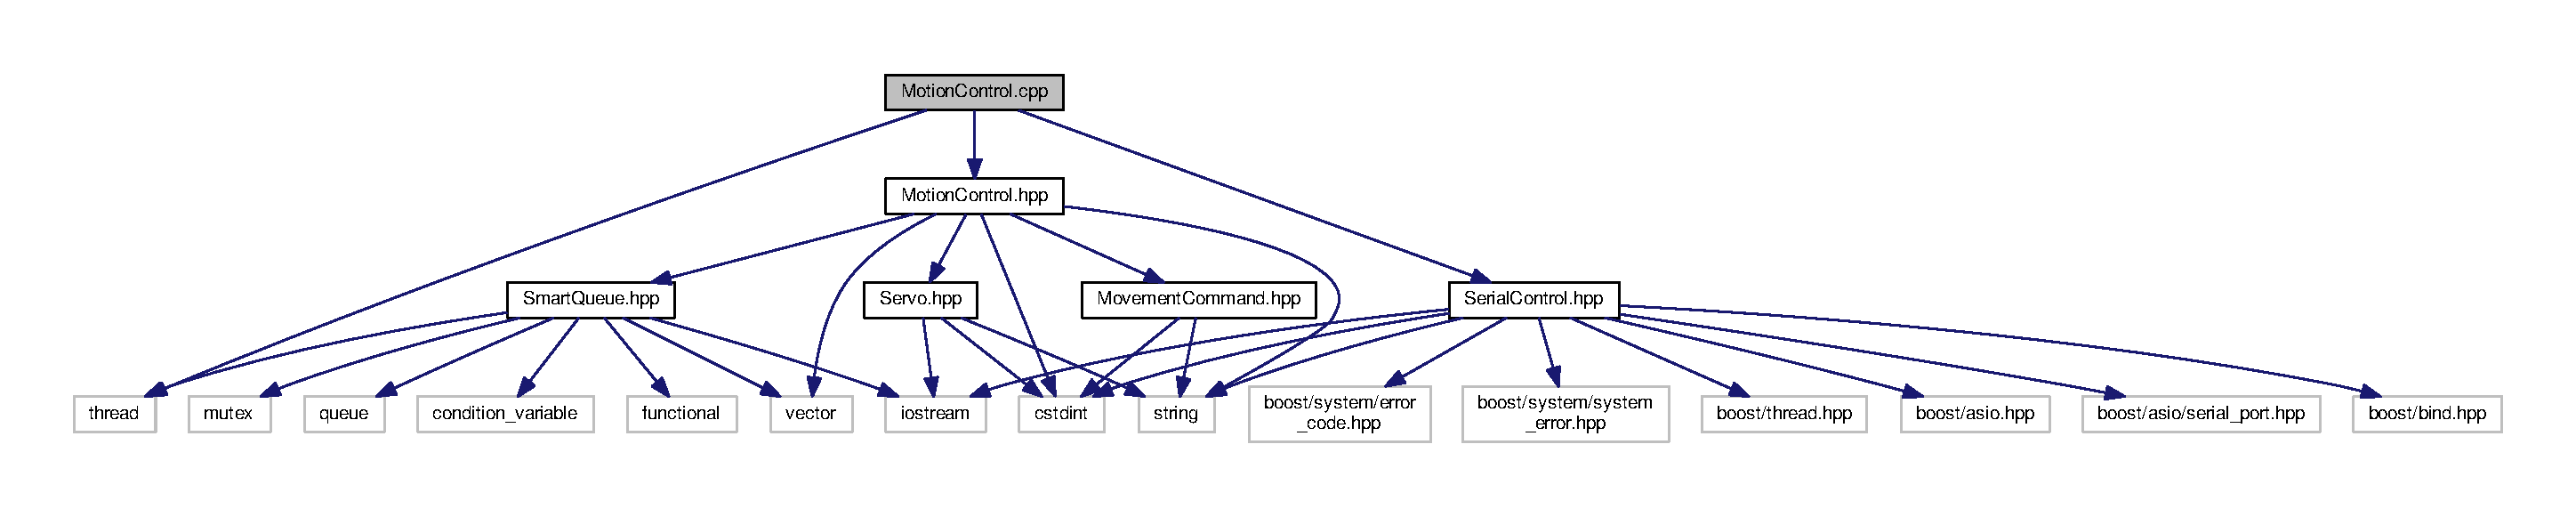
\includegraphics[width=350pt]{_motion_control_8cpp__incl}
\end{center}
\end{figure}

\hypertarget{_motion_control_8hpp}{}\section{Motion\+Control.\+hpp File Reference}
\label{_motion_control_8hpp}\index{Motion\+Control.\+hpp@{Motion\+Control.\+hpp}}
{\ttfamily \#include \char`\"{}Movement\+Command.\+hpp\char`\"{}}\\*
{\ttfamily \#include \char`\"{}Servo.\+hpp\char`\"{}}\\*
{\ttfamily \#include \char`\"{}Smart\+Queue.\+hpp\char`\"{}}\\*
{\ttfamily \#include $<$cstdint$>$}\\*
{\ttfamily \#include $<$string$>$}\\*
{\ttfamily \#include $<$vector$>$}\\*
Include dependency graph for Motion\+Control.\+hpp\+:
\nopagebreak
\begin{figure}[H]
\begin{center}
\leavevmode
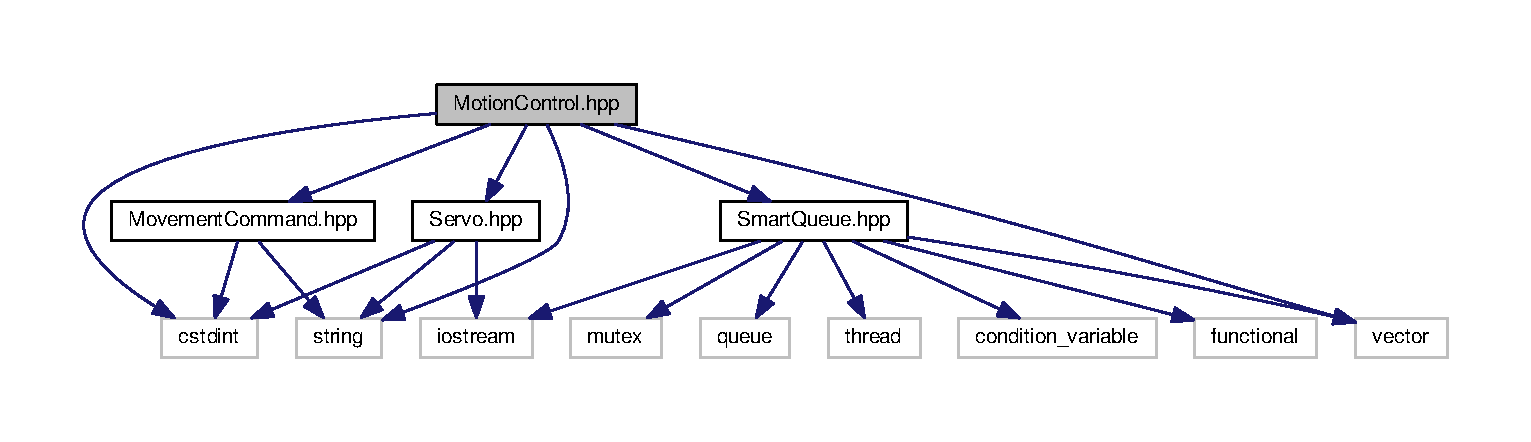
\includegraphics[width=350pt]{_motion_control_8hpp__incl}
\end{center}
\end{figure}
\subsection*{Classes}
\begin{DoxyCompactItemize}
\item 
class \hyperlink{class_motion_control}{Motion\+Control}
\end{DoxyCompactItemize}
\subsection*{Macros}
\begin{DoxyCompactItemize}
\item 
\#define \hyperlink{_motion_control_8hpp_a4a70d629781891dfddbb5caaff3254b0}{M\+A\+X\+\_\+\+S\+T\+A\+R\+T\+U\+P\+\_\+\+S\+T\+R\+I\+N\+G\+\_\+\+L\+E\+N\+G\+TH}~100
\end{DoxyCompactItemize}
\subsection*{Enumerations}
\begin{DoxyCompactItemize}
\item 
enum \hyperlink{_motion_control_8hpp_ac70e3c2821eb6a3860441f2c682f0aa4}{default\+Positions} \{ \hyperlink{_motion_control_8hpp_ac70e3c2821eb6a3860441f2c682f0aa4ad22433eb60c8f12c80d3f45d02709b7b}{P\+A\+RK}, 
\hyperlink{_motion_control_8hpp_ac70e3c2821eb6a3860441f2c682f0aa4a6564f2f3e15be06b670547bbcaaf0798}{R\+E\+A\+DY}, 
\hyperlink{_motion_control_8hpp_ac70e3c2821eb6a3860441f2c682f0aa4af5805c05649c241ed1abb43be8aec4fd}{S\+T\+R\+A\+I\+G\+H\+T\+\_\+\+UP}
 \}
\item 
enum \hyperlink{_motion_control_8hpp_ac095d62e5392b8d263c10f37a76e6d9b}{interface\+States} \{ \\*
\hyperlink{_motion_control_8hpp_ac095d62e5392b8d263c10f37a76e6d9bafd6a0e4343048b10646dd2976cc5ad18}{I\+D\+LE}, 
\hyperlink{_motion_control_8hpp_ac095d62e5392b8d263c10f37a76e6d9bae60eddad476ae478c84c809abc870c43}{S\+E\+N\+D\+I\+N\+G\+\_\+\+C\+O\+M\+M\+A\+ND}, 
\hyperlink{_motion_control_8hpp_ac095d62e5392b8d263c10f37a76e6d9ba4a9519c547008a358feb79d802607f8f}{M\+O\+V\+I\+N\+G\+\_\+\+A\+RM}, 
\hyperlink{_motion_control_8hpp_ac095d62e5392b8d263c10f37a76e6d9ba4b8a0c31ecac9e76c03a10bb451b8fe8}{M\+O\+V\+I\+N\+G\+\_\+\+F\+I\+N\+I\+S\+H\+ED}, 
\\*
\hyperlink{_motion_control_8hpp_ac095d62e5392b8d263c10f37a76e6d9ba0cb1b2c6a7db1f1084886c98909a3f36}{I\+N\+IT}, 
\hyperlink{_motion_control_8hpp_ac095d62e5392b8d263c10f37a76e6d9baa446325b29d7c917325acc576f0f0f45}{I\+N\+I\+T\+\_\+\+E\+R\+R\+OR}, 
\hyperlink{_motion_control_8hpp_ac095d62e5392b8d263c10f37a76e6d9ba56a92b9980c854fa6e488ffeb6a2844b}{E\+M\+E\+R\+G\+E\+N\+C\+Y\+\_\+\+S\+T\+OP}
 \}
\end{DoxyCompactItemize}


\subsection{Macro Definition Documentation}
\index{Motion\+Control.\+hpp@{Motion\+Control.\+hpp}!M\+A\+X\+\_\+\+S\+T\+A\+R\+T\+U\+P\+\_\+\+S\+T\+R\+I\+N\+G\+\_\+\+L\+E\+N\+G\+TH@{M\+A\+X\+\_\+\+S\+T\+A\+R\+T\+U\+P\+\_\+\+S\+T\+R\+I\+N\+G\+\_\+\+L\+E\+N\+G\+TH}}
\index{M\+A\+X\+\_\+\+S\+T\+A\+R\+T\+U\+P\+\_\+\+S\+T\+R\+I\+N\+G\+\_\+\+L\+E\+N\+G\+TH@{M\+A\+X\+\_\+\+S\+T\+A\+R\+T\+U\+P\+\_\+\+S\+T\+R\+I\+N\+G\+\_\+\+L\+E\+N\+G\+TH}!Motion\+Control.\+hpp@{Motion\+Control.\+hpp}}
\subsubsection[{\texorpdfstring{M\+A\+X\+\_\+\+S\+T\+A\+R\+T\+U\+P\+\_\+\+S\+T\+R\+I\+N\+G\+\_\+\+L\+E\+N\+G\+TH}{MAX_STARTUP_STRING_LENGTH}}]{\setlength{\rightskip}{0pt plus 5cm}\#define M\+A\+X\+\_\+\+S\+T\+A\+R\+T\+U\+P\+\_\+\+S\+T\+R\+I\+N\+G\+\_\+\+L\+E\+N\+G\+TH~100}\hypertarget{_motion_control_8hpp_a4a70d629781891dfddbb5caaff3254b0}{}\label{_motion_control_8hpp_a4a70d629781891dfddbb5caaff3254b0}


\subsection{Enumeration Type Documentation}
\index{Motion\+Control.\+hpp@{Motion\+Control.\+hpp}!default\+Positions@{default\+Positions}}
\index{default\+Positions@{default\+Positions}!Motion\+Control.\+hpp@{Motion\+Control.\+hpp}}
\subsubsection[{\texorpdfstring{default\+Positions}{defaultPositions}}]{\setlength{\rightskip}{0pt plus 5cm}enum {\bf default\+Positions}}\hypertarget{_motion_control_8hpp_ac70e3c2821eb6a3860441f2c682f0aa4}{}\label{_motion_control_8hpp_ac70e3c2821eb6a3860441f2c682f0aa4}
\begin{Desc}
\item[Enumerator]\par
\begin{description}
\index{P\+A\+RK@{P\+A\+RK}!Motion\+Control.\+hpp@{Motion\+Control.\+hpp}}\index{Motion\+Control.\+hpp@{Motion\+Control.\+hpp}!P\+A\+RK@{P\+A\+RK}}\item[{\em 
P\+A\+RK\hypertarget{_motion_control_8hpp_ac70e3c2821eb6a3860441f2c682f0aa4ad22433eb60c8f12c80d3f45d02709b7b}{}\label{_motion_control_8hpp_ac70e3c2821eb6a3860441f2c682f0aa4ad22433eb60c8f12c80d3f45d02709b7b}
}]\index{R\+E\+A\+DY@{R\+E\+A\+DY}!Motion\+Control.\+hpp@{Motion\+Control.\+hpp}}\index{Motion\+Control.\+hpp@{Motion\+Control.\+hpp}!R\+E\+A\+DY@{R\+E\+A\+DY}}\item[{\em 
R\+E\+A\+DY\hypertarget{_motion_control_8hpp_ac70e3c2821eb6a3860441f2c682f0aa4a6564f2f3e15be06b670547bbcaaf0798}{}\label{_motion_control_8hpp_ac70e3c2821eb6a3860441f2c682f0aa4a6564f2f3e15be06b670547bbcaaf0798}
}]\index{S\+T\+R\+A\+I\+G\+H\+T\+\_\+\+UP@{S\+T\+R\+A\+I\+G\+H\+T\+\_\+\+UP}!Motion\+Control.\+hpp@{Motion\+Control.\+hpp}}\index{Motion\+Control.\+hpp@{Motion\+Control.\+hpp}!S\+T\+R\+A\+I\+G\+H\+T\+\_\+\+UP@{S\+T\+R\+A\+I\+G\+H\+T\+\_\+\+UP}}\item[{\em 
S\+T\+R\+A\+I\+G\+H\+T\+\_\+\+UP\hypertarget{_motion_control_8hpp_ac70e3c2821eb6a3860441f2c682f0aa4af5805c05649c241ed1abb43be8aec4fd}{}\label{_motion_control_8hpp_ac70e3c2821eb6a3860441f2c682f0aa4af5805c05649c241ed1abb43be8aec4fd}
}]\end{description}
\end{Desc}
\index{Motion\+Control.\+hpp@{Motion\+Control.\+hpp}!interface\+States@{interface\+States}}
\index{interface\+States@{interface\+States}!Motion\+Control.\+hpp@{Motion\+Control.\+hpp}}
\subsubsection[{\texorpdfstring{interface\+States}{interfaceStates}}]{\setlength{\rightskip}{0pt plus 5cm}enum {\bf interface\+States}}\hypertarget{_motion_control_8hpp_ac095d62e5392b8d263c10f37a76e6d9b}{}\label{_motion_control_8hpp_ac095d62e5392b8d263c10f37a76e6d9b}
\begin{Desc}
\item[Enumerator]\par
\begin{description}
\index{I\+D\+LE@{I\+D\+LE}!Motion\+Control.\+hpp@{Motion\+Control.\+hpp}}\index{Motion\+Control.\+hpp@{Motion\+Control.\+hpp}!I\+D\+LE@{I\+D\+LE}}\item[{\em 
I\+D\+LE\hypertarget{_motion_control_8hpp_ac095d62e5392b8d263c10f37a76e6d9bafd6a0e4343048b10646dd2976cc5ad18}{}\label{_motion_control_8hpp_ac095d62e5392b8d263c10f37a76e6d9bafd6a0e4343048b10646dd2976cc5ad18}
}]\index{S\+E\+N\+D\+I\+N\+G\+\_\+\+C\+O\+M\+M\+A\+ND@{S\+E\+N\+D\+I\+N\+G\+\_\+\+C\+O\+M\+M\+A\+ND}!Motion\+Control.\+hpp@{Motion\+Control.\+hpp}}\index{Motion\+Control.\+hpp@{Motion\+Control.\+hpp}!S\+E\+N\+D\+I\+N\+G\+\_\+\+C\+O\+M\+M\+A\+ND@{S\+E\+N\+D\+I\+N\+G\+\_\+\+C\+O\+M\+M\+A\+ND}}\item[{\em 
S\+E\+N\+D\+I\+N\+G\+\_\+\+C\+O\+M\+M\+A\+ND\hypertarget{_motion_control_8hpp_ac095d62e5392b8d263c10f37a76e6d9bae60eddad476ae478c84c809abc870c43}{}\label{_motion_control_8hpp_ac095d62e5392b8d263c10f37a76e6d9bae60eddad476ae478c84c809abc870c43}
}]\index{M\+O\+V\+I\+N\+G\+\_\+\+A\+RM@{M\+O\+V\+I\+N\+G\+\_\+\+A\+RM}!Motion\+Control.\+hpp@{Motion\+Control.\+hpp}}\index{Motion\+Control.\+hpp@{Motion\+Control.\+hpp}!M\+O\+V\+I\+N\+G\+\_\+\+A\+RM@{M\+O\+V\+I\+N\+G\+\_\+\+A\+RM}}\item[{\em 
M\+O\+V\+I\+N\+G\+\_\+\+A\+RM\hypertarget{_motion_control_8hpp_ac095d62e5392b8d263c10f37a76e6d9ba4a9519c547008a358feb79d802607f8f}{}\label{_motion_control_8hpp_ac095d62e5392b8d263c10f37a76e6d9ba4a9519c547008a358feb79d802607f8f}
}]\index{M\+O\+V\+I\+N\+G\+\_\+\+F\+I\+N\+I\+S\+H\+ED@{M\+O\+V\+I\+N\+G\+\_\+\+F\+I\+N\+I\+S\+H\+ED}!Motion\+Control.\+hpp@{Motion\+Control.\+hpp}}\index{Motion\+Control.\+hpp@{Motion\+Control.\+hpp}!M\+O\+V\+I\+N\+G\+\_\+\+F\+I\+N\+I\+S\+H\+ED@{M\+O\+V\+I\+N\+G\+\_\+\+F\+I\+N\+I\+S\+H\+ED}}\item[{\em 
M\+O\+V\+I\+N\+G\+\_\+\+F\+I\+N\+I\+S\+H\+ED\hypertarget{_motion_control_8hpp_ac095d62e5392b8d263c10f37a76e6d9ba4b8a0c31ecac9e76c03a10bb451b8fe8}{}\label{_motion_control_8hpp_ac095d62e5392b8d263c10f37a76e6d9ba4b8a0c31ecac9e76c03a10bb451b8fe8}
}]\index{I\+N\+IT@{I\+N\+IT}!Motion\+Control.\+hpp@{Motion\+Control.\+hpp}}\index{Motion\+Control.\+hpp@{Motion\+Control.\+hpp}!I\+N\+IT@{I\+N\+IT}}\item[{\em 
I\+N\+IT\hypertarget{_motion_control_8hpp_ac095d62e5392b8d263c10f37a76e6d9ba0cb1b2c6a7db1f1084886c98909a3f36}{}\label{_motion_control_8hpp_ac095d62e5392b8d263c10f37a76e6d9ba0cb1b2c6a7db1f1084886c98909a3f36}
}]\index{I\+N\+I\+T\+\_\+\+E\+R\+R\+OR@{I\+N\+I\+T\+\_\+\+E\+R\+R\+OR}!Motion\+Control.\+hpp@{Motion\+Control.\+hpp}}\index{Motion\+Control.\+hpp@{Motion\+Control.\+hpp}!I\+N\+I\+T\+\_\+\+E\+R\+R\+OR@{I\+N\+I\+T\+\_\+\+E\+R\+R\+OR}}\item[{\em 
I\+N\+I\+T\+\_\+\+E\+R\+R\+OR\hypertarget{_motion_control_8hpp_ac095d62e5392b8d263c10f37a76e6d9baa446325b29d7c917325acc576f0f0f45}{}\label{_motion_control_8hpp_ac095d62e5392b8d263c10f37a76e6d9baa446325b29d7c917325acc576f0f0f45}
}]\index{E\+M\+E\+R\+G\+E\+N\+C\+Y\+\_\+\+S\+T\+OP@{E\+M\+E\+R\+G\+E\+N\+C\+Y\+\_\+\+S\+T\+OP}!Motion\+Control.\+hpp@{Motion\+Control.\+hpp}}\index{Motion\+Control.\+hpp@{Motion\+Control.\+hpp}!E\+M\+E\+R\+G\+E\+N\+C\+Y\+\_\+\+S\+T\+OP@{E\+M\+E\+R\+G\+E\+N\+C\+Y\+\_\+\+S\+T\+OP}}\item[{\em 
E\+M\+E\+R\+G\+E\+N\+C\+Y\+\_\+\+S\+T\+OP\hypertarget{_motion_control_8hpp_ac095d62e5392b8d263c10f37a76e6d9ba56a92b9980c854fa6e488ffeb6a2844b}{}\label{_motion_control_8hpp_ac095d62e5392b8d263c10f37a76e6d9ba56a92b9980c854fa6e488ffeb6a2844b}
}]\end{description}
\end{Desc}

\hypertarget{_movement_command_8hpp}{}\section{Movement\+Command.\+hpp File Reference}
\label{_movement_command_8hpp}\index{Movement\+Command.\+hpp@{Movement\+Command.\+hpp}}
{\ttfamily \#include $<$cstdint$>$}\\*
{\ttfamily \#include $<$string$>$}\\*
Include dependency graph for Movement\+Command.\+hpp\+:
\nopagebreak
\begin{figure}[H]
\begin{center}
\leavevmode
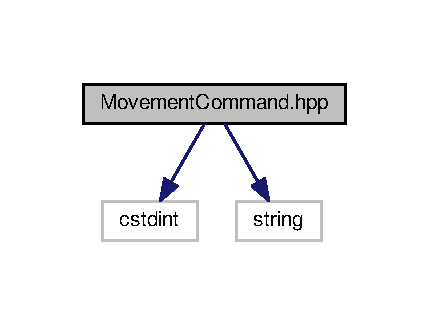
\includegraphics[width=206pt]{_movement_command_8hpp__incl}
\end{center}
\end{figure}
\subsection*{Classes}
\begin{DoxyCompactItemize}
\item 
class \hyperlink{class_movement_command}{Movement\+Command}
\end{DoxyCompactItemize}

\hypertarget{_ros_communication_8cpp}{}\section{Ros\+Communication.\+cpp File Reference}
\label{_ros_communication_8cpp}\index{Ros\+Communication.\+cpp@{Ros\+Communication.\+cpp}}
{\ttfamily \#include \char`\"{}Ros\+Communication.\+hpp\char`\"{}}\\*
{\ttfamily \#include $<$boost/algorithm/string.\+hpp$>$}\\*
Include dependency graph for Ros\+Communication.\+cpp\+:
\nopagebreak
\begin{figure}[H]
\begin{center}
\leavevmode
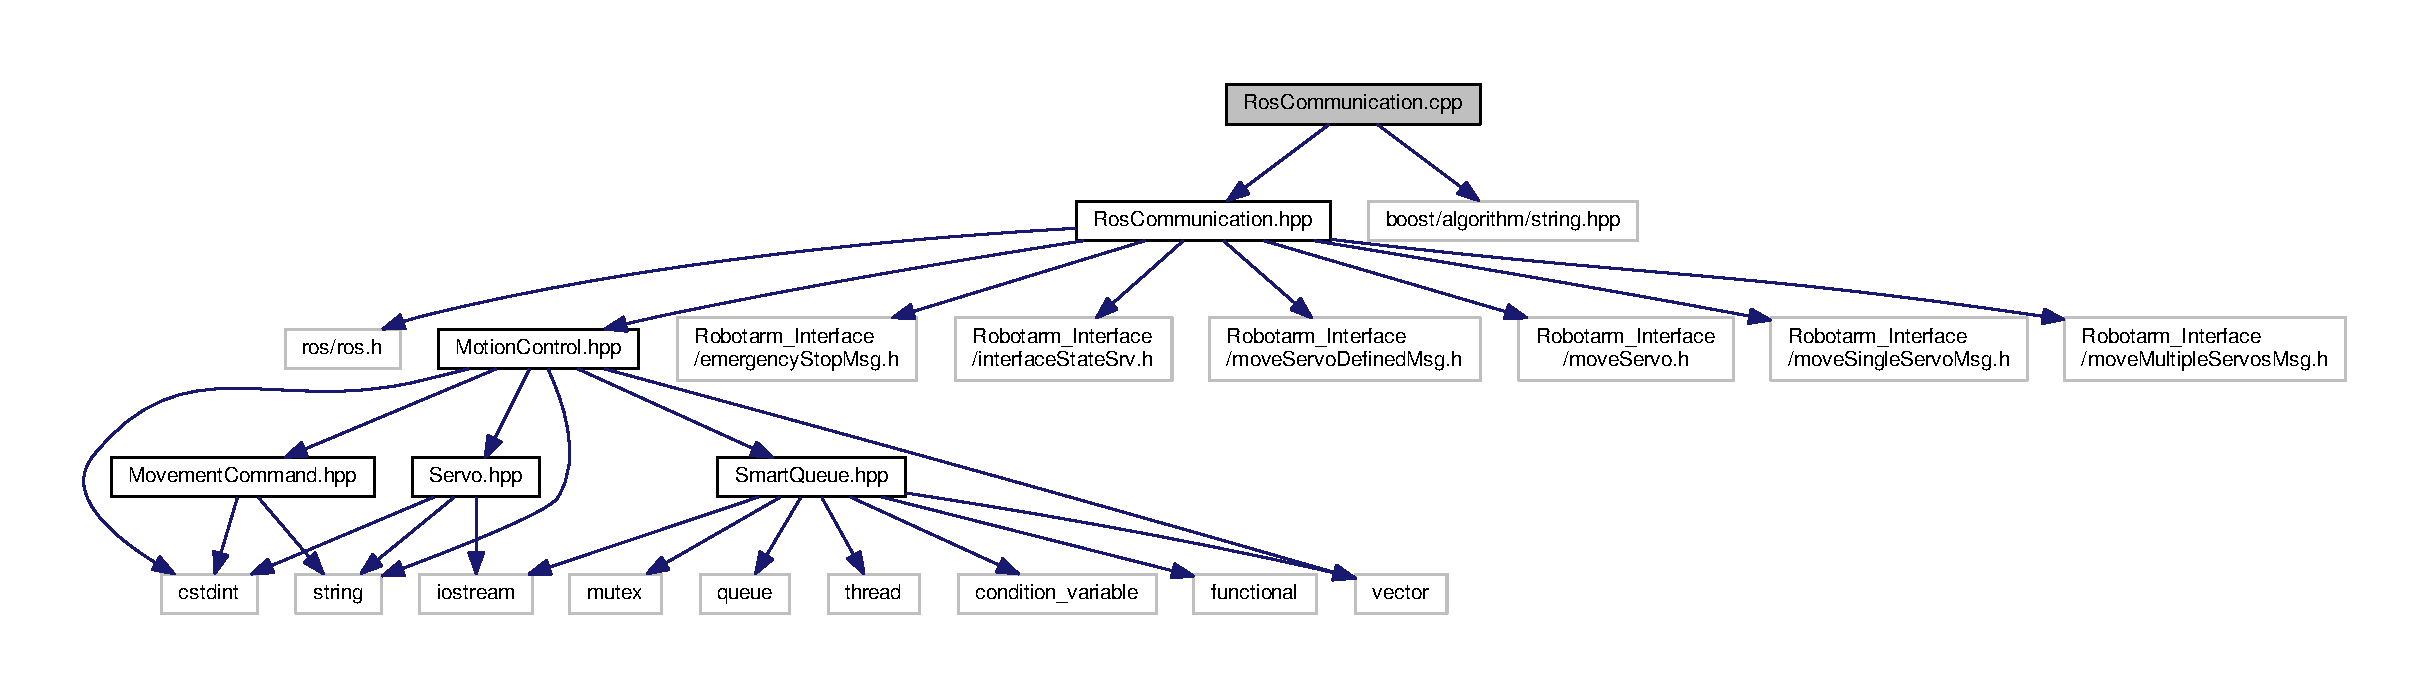
\includegraphics[width=350pt]{_ros_communication_8cpp__incl}
\end{center}
\end{figure}

\hypertarget{_ros_communication_8hpp}{}\section{Ros\+Communication.\+hpp File Reference}
\label{_ros_communication_8hpp}\index{Ros\+Communication.\+hpp@{Ros\+Communication.\+hpp}}
{\ttfamily \#include \char`\"{}ros/ros.\+h\char`\"{}}\\*
{\ttfamily \#include \char`\"{}Motion\+Control.\+hpp\char`\"{}}\\*
{\ttfamily \#include \char`\"{}Robotarm\+\_\+\+Interface/emergency\+Stop\+Msg.\+h\char`\"{}}\\*
{\ttfamily \#include \char`\"{}Robotarm\+\_\+\+Interface/interface\+State\+Srv.\+h\char`\"{}}\\*
{\ttfamily \#include \char`\"{}Robotarm\+\_\+\+Interface/move\+Servo\+Defined\+Msg.\+h\char`\"{}}\\*
{\ttfamily \#include \char`\"{}Robotarm\+\_\+\+Interface/move\+Servo.\+h\char`\"{}}\\*
{\ttfamily \#include \char`\"{}Robotarm\+\_\+\+Interface/move\+Single\+Servo\+Msg.\+h\char`\"{}}\\*
{\ttfamily \#include \char`\"{}Robotarm\+\_\+\+Interface/move\+Multiple\+Servos\+Msg.\+h\char`\"{}}\\*
Include dependency graph for Ros\+Communication.\+hpp\+:
\nopagebreak
\begin{figure}[H]
\begin{center}
\leavevmode
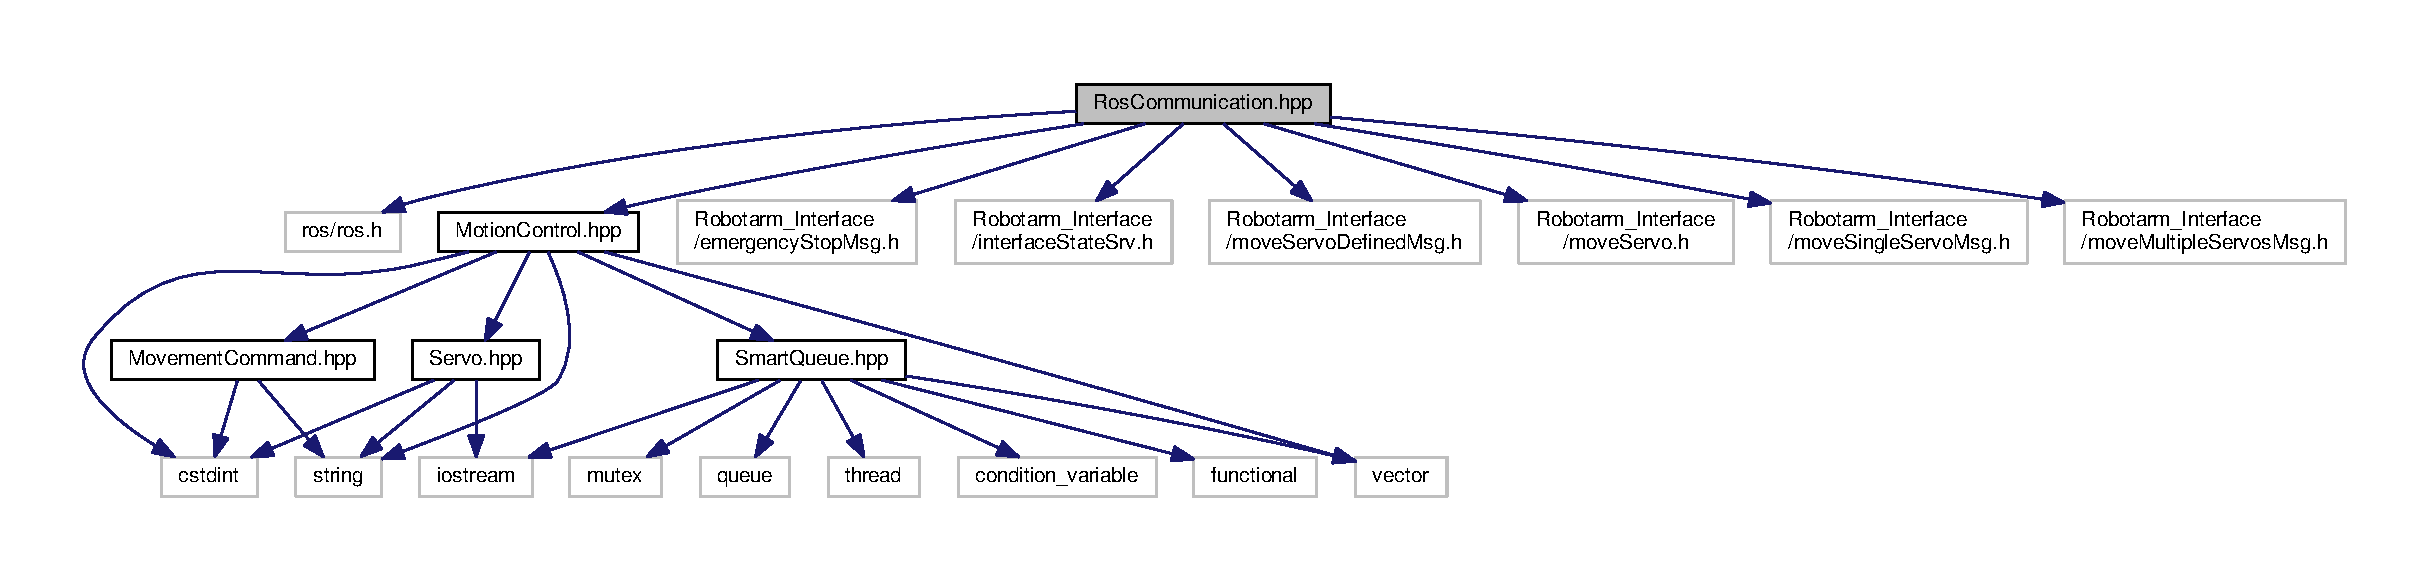
\includegraphics[width=350pt]{_ros_communication_8hpp__incl}
\end{center}
\end{figure}
\subsection*{Classes}
\begin{DoxyCompactItemize}
\item 
class \hyperlink{class_ros_communication}{Ros\+Communication}
\end{DoxyCompactItemize}

\hypertarget{_serial_control_8cpp}{}\section{Serial\+Control.\+cpp File Reference}
\label{_serial_control_8cpp}\index{Serial\+Control.\+cpp@{Serial\+Control.\+cpp}}
{\ttfamily \#include \char`\"{}Serial\+Control.\+hpp\char`\"{}}\\*
Include dependency graph for Serial\+Control.\+cpp\+:
\nopagebreak
\begin{figure}[H]
\begin{center}
\leavevmode
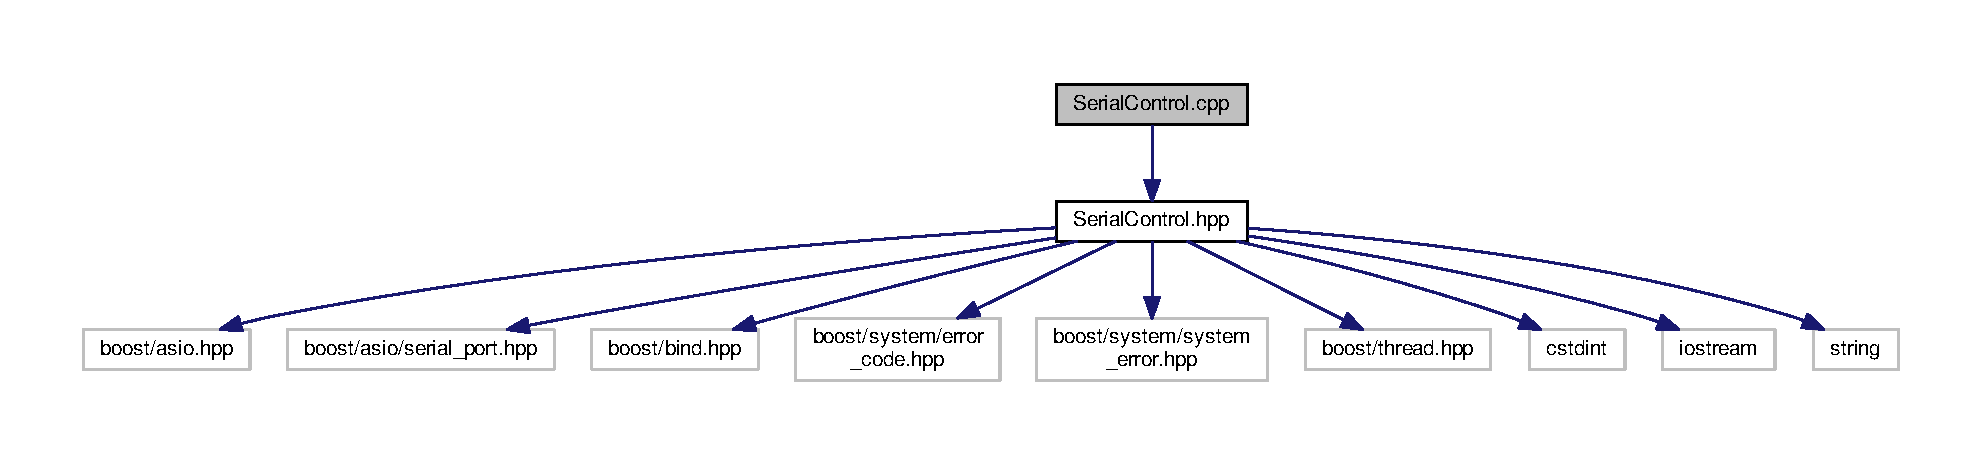
\includegraphics[width=350pt]{_serial_control_8cpp__incl}
\end{center}
\end{figure}

\hypertarget{_serial_control_8hpp}{}\section{Serial\+Control.\+hpp File Reference}
\label{_serial_control_8hpp}\index{Serial\+Control.\+hpp@{Serial\+Control.\+hpp}}
{\ttfamily \#include $<$boost/asio.\+hpp$>$}\\*
{\ttfamily \#include $<$boost/asio/serial\+\_\+port.\+hpp$>$}\\*
{\ttfamily \#include $<$boost/bind.\+hpp$>$}\\*
{\ttfamily \#include $<$boost/system/error\+\_\+code.\+hpp$>$}\\*
{\ttfamily \#include $<$boost/system/system\+\_\+error.\+hpp$>$}\\*
{\ttfamily \#include $<$boost/thread.\+hpp$>$}\\*
{\ttfamily \#include $<$cstdint$>$}\\*
{\ttfamily \#include $<$iostream$>$}\\*
{\ttfamily \#include $<$string$>$}\\*
Include dependency graph for Serial\+Control.\+hpp\+:
\nopagebreak
\begin{figure}[H]
\begin{center}
\leavevmode
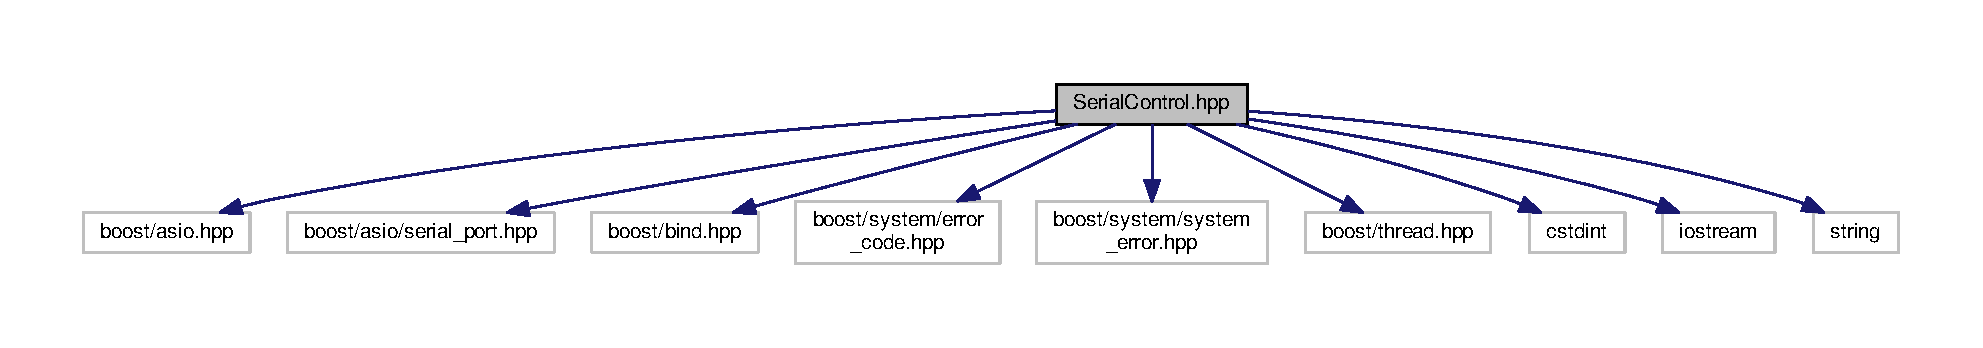
\includegraphics[width=350pt]{_serial_control_8hpp__incl}
\end{center}
\end{figure}
\subsection*{Classes}
\begin{DoxyCompactItemize}
\item 
class \hyperlink{class_serial_control}{Serial\+Control}
\end{DoxyCompactItemize}
\subsection*{Macros}
\begin{DoxyCompactItemize}
\item 
\#define \hyperlink{_serial_control_8hpp_a46167a977503a51eb6efe97e870568c3}{R\+E\+A\+D\+\_\+\+B\+U\+F\+F\+E\+R\+\_\+\+S\+I\+ZE}~256
\end{DoxyCompactItemize}
\subsection*{Typedefs}
\begin{DoxyCompactItemize}
\item 
typedef boost\+::shared\+\_\+ptr$<$ boost\+::asio\+::serial\+\_\+port $>$ \hyperlink{_serial_control_8hpp_afb8bc9337e0426063f723bb57bfa1055}{serial\+\_\+port\+\_\+ptr}
\end{DoxyCompactItemize}


\subsection{Macro Definition Documentation}
\index{Serial\+Control.\+hpp@{Serial\+Control.\+hpp}!R\+E\+A\+D\+\_\+\+B\+U\+F\+F\+E\+R\+\_\+\+S\+I\+ZE@{R\+E\+A\+D\+\_\+\+B\+U\+F\+F\+E\+R\+\_\+\+S\+I\+ZE}}
\index{R\+E\+A\+D\+\_\+\+B\+U\+F\+F\+E\+R\+\_\+\+S\+I\+ZE@{R\+E\+A\+D\+\_\+\+B\+U\+F\+F\+E\+R\+\_\+\+S\+I\+ZE}!Serial\+Control.\+hpp@{Serial\+Control.\+hpp}}
\subsubsection[{\texorpdfstring{R\+E\+A\+D\+\_\+\+B\+U\+F\+F\+E\+R\+\_\+\+S\+I\+ZE}{READ_BUFFER_SIZE}}]{\setlength{\rightskip}{0pt plus 5cm}\#define R\+E\+A\+D\+\_\+\+B\+U\+F\+F\+E\+R\+\_\+\+S\+I\+ZE~256}\hypertarget{_serial_control_8hpp_a46167a977503a51eb6efe97e870568c3}{}\label{_serial_control_8hpp_a46167a977503a51eb6efe97e870568c3}


\subsection{Typedef Documentation}
\index{Serial\+Control.\+hpp@{Serial\+Control.\+hpp}!serial\+\_\+port\+\_\+ptr@{serial\+\_\+port\+\_\+ptr}}
\index{serial\+\_\+port\+\_\+ptr@{serial\+\_\+port\+\_\+ptr}!Serial\+Control.\+hpp@{Serial\+Control.\+hpp}}
\subsubsection[{\texorpdfstring{serial\+\_\+port\+\_\+ptr}{serial_port_ptr}}]{\setlength{\rightskip}{0pt plus 5cm}typedef boost\+::shared\+\_\+ptr$<$boost\+::asio\+::serial\+\_\+port$>$ {\bf serial\+\_\+port\+\_\+ptr}}\hypertarget{_serial_control_8hpp_afb8bc9337e0426063f723bb57bfa1055}{}\label{_serial_control_8hpp_afb8bc9337e0426063f723bb57bfa1055}

\hypertarget{_servo_8hpp}{}\section{Servo.\+hpp File Reference}
\label{_servo_8hpp}\index{Servo.\+hpp@{Servo.\+hpp}}
{\ttfamily \#include $<$cstdint$>$}\\*
{\ttfamily \#include $<$iostream$>$}\\*
{\ttfamily \#include $<$string$>$}\\*
Include dependency graph for Servo.\+hpp\+:
\nopagebreak
\begin{figure}[H]
\begin{center}
\leavevmode
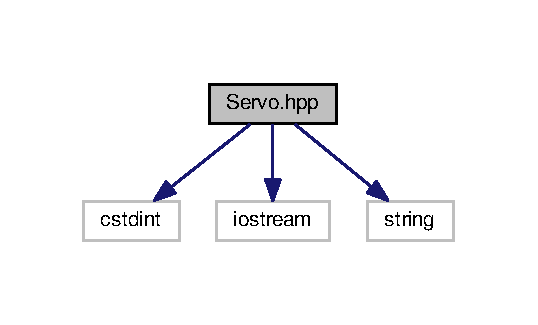
\includegraphics[width=258pt]{_servo_8hpp__incl}
\end{center}
\end{figure}
\subsection*{Classes}
\begin{DoxyCompactItemize}
\item 
class \hyperlink{class_servo}{Servo}
\end{DoxyCompactItemize}

\hypertarget{_smart_queue_8hpp}{}\section{Smart\+Queue.\+hpp File Reference}
\label{_smart_queue_8hpp}\index{Smart\+Queue.\+hpp@{Smart\+Queue.\+hpp}}
{\ttfamily \#include $<$condition\+\_\+variable$>$}\\*
{\ttfamily \#include $<$functional$>$}\\*
{\ttfamily \#include $<$iostream$>$}\\*
{\ttfamily \#include $<$mutex$>$}\\*
{\ttfamily \#include $<$queue$>$}\\*
{\ttfamily \#include $<$thread$>$}\\*
{\ttfamily \#include $<$vector$>$}\\*
Include dependency graph for Smart\+Queue.\+hpp\+:
\nopagebreak
\begin{figure}[H]
\begin{center}
\leavevmode
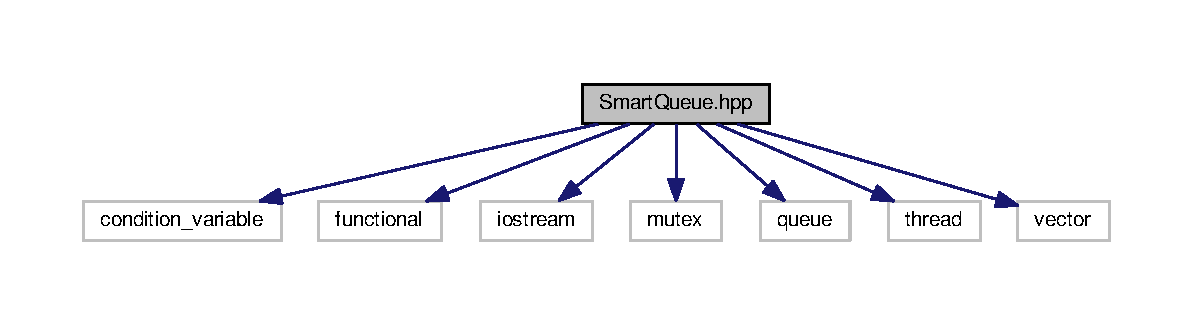
\includegraphics[width=350pt]{_smart_queue_8hpp__incl}
\end{center}
\end{figure}
\subsection*{Classes}
\begin{DoxyCompactItemize}
\item 
class \hyperlink{class_smart_queue}{Smart\+Queue$<$ T $>$}
\end{DoxyCompactItemize}

%--- End generated contents ---

% Index
\backmatter
\newpage
\phantomsection
\clearemptydoublepage
\addcontentsline{toc}{chapter}{Index}
\printindex

\end{document}
